%% abtex2-modelo-trabalho-academico.tex, v-1.9.5 laurocesar
%% Copyright 2012-2015 by abnTeX2 group at http://www.abntex.net.br/ 
%%
%% This work may be distributed and/or modified under the
%% conditions of the LaTeX Project Public License, either version 1.3
%% of this license or (at your option) any later version.
%% The latest version of this license is in
%%   http://www.latex-project.org/lppl.txt
%% and version 1.3 or later is part of all distributions of LaTeX
%% version 2005/12/01 or later.
%%
%% This work has the LPPL maintenance status `maintained'.
%% 
%% The Current Maintainer of this work is the abnTeX2 team, led
%% by Lauro César Araujo. Further information are available on 
%% http://www.abntex.net.br/
%%
%% This work consists of the files abntex2-modelo-trabalho-academico.tex,
%% abntex2-modelo-include-comandos and abntex2-modelo-references.bib
%%

% ------------------------------------------------------------------------
% ------------------------------------------------------------------------
% abnTeX2: Modelo de Trabalho Academico (tese de doutorado, dissertacao de
% mestrado e trabalhos monograficos em geral) em conformidade com 
% ABNT NBR 14724:2011: Informacao e documentacao - Trabalhos academicos -
% Apresentacao
% ------------------------------------------------------------------------
% ------------------------------------------------------------------------

\documentclass[
	% -- opções da classe memoir --
	12pt,				% tamanho da fonte
	openright,			% capítulos começam em pág ímpar (insere página vazia caso preciso)
	twoside,			% para impressão em verso e anverso. Oposto a oneside
	a4paper,			% tamanho do papel. 
	% -- opções da classe abntex2 --
	%chapter=TITLE,		% títulos de capítulos convertidos em letras maiúsculas
	%section=TITLE,		% títulos de seções convertidos em letras maiúsculas
	%subsection=TITLE,	% títulos de subseções convertidos em letras maiúsculas
    %subsubsection=TITLE,% títulos de subsubseções convertidos em letras maiúsculas
	% -- opções do pacote babel --
	english,			% idioma adicional para hifenização
	french,				% idioma adicional para hifenização
	spanish,			% idioma adicional para hifenização
	brazil				% o último idioma é o principal do documento
	]{abntex2}

% ---
% Pacotes básicos 
% ---
\usepackage{lmodern}			% Usa a fonte Latin Modern			
\usepackage[T1]{fontenc}		% Selecao de codigos de fonte.
\usepackage[utf8]{inputenc}		% Codificacao do documento (conversão automática dos acentos)
\usepackage{lastpage}			% Usado pela Ficha catalográfica
\usepackage{indentfirst}		% Indenta o primeiro parágrafo de cada seção.
\usepackage{color}				% Controle das cores
\usepackage{graphicx}			% Inclusão de gráficos
\usepackage{microtype} 			% para melhorias de justificação
\usepackage{amsmath}            % Matrizes e fórmulas matemáticas (customizado)
\usepackage{mathtools}
% ---
		
% ---
% Pacotes adicionais, usados apenas no âmbito do Modelo Canônico do abnteX2
% ---
\usepackage{lipsum}				% para geração de dummy text
% ---

% ---
% Pacotes de citações
% ---
\usepackage[brazilian,hyperpageref]{backref}	 % Paginas com as citações na bibl
\usepackage[alf]{abntex2cite}	% Citações padrão ABNT

% --- 
% CONFIGURAÇÕES DE PACOTES
% --- 

% ---
% Configurações do pacote backref
% Usado sem a opção hyperpageref de backref
\renewcommand{\backrefpagesname}{Citado na(s) página(s):~}
% Texto padrão antes do número das páginas
\renewcommand{\backref}{}
% Define os textos da citação
\renewcommand*{\backrefalt}[4]{
	\ifcase #1 %
		Nenhuma citação no texto.%
	\or
		Citado na página #2.%
	\else
		Citado #1 vezes nas páginas #2.%
	\fi}%
% ---

% ---
% Informações de dados para CAPA e FOLHA DE ROSTO
% ---
\titulo{Trabalho de Conclusão de Curso - Identificação de Parâmetros através de Sinal Persistentemente Excitante com Esquema de Desligamento Automático}
\autor{Pedro Yochinori Gushiken}
\local{Brasil}
\data{2015, v-0.4}
\orientador{Aldayr Dantas de Araújo}
\instituicao{%
  Universidade Federal do Rio Grande do Norte -- UFRN
  \par
  Departamento de Engenharia Elétrica
  \par
  Programa de Graduação}
\tipotrabalho{TCC}
% O preambulo deve conter o tipo do trabalho, o objetivo, 
% o nome da instituição e a área de concentração 
\preambulo{Uso de estratégias de identificação de parâmetros com sinal Persistentemente Excitante(PE) onde o objetivo é explicitamente alcançar a convergência das estimativas e o desligamento do sinal PE.}
% ---


% ---
% Configurações de aparência do PDF final

% alterando o aspecto da cor azul
\definecolor{blue}{RGB}{41,5,195}

% informações do PDF
\makeatletter
\hypersetup{
     	%pagebackref=true,
		pdftitle={\@title}, 
		pdfauthor={\@author},
    	pdfsubject={\imprimirpreambulo},
	    pdfcreator={LaTeX with abnTeX2},
		pdfkeywords={abnt}{latex}{abntex}{abntex2}{trabalho acadêmico}, 
		colorlinks=true,       		% false: boxed links; true: colored links
    	linkcolor=blue,          	% color of internal links
    	citecolor=blue,        		% color of links to bibliography
    	filecolor=magenta,      		% color of file links
		urlcolor=blue,
		bookmarksdepth=4
}
\makeatother
% --- 

% --- 
% Espaçamentos entre linhas e parágrafos 
% --- 

% O tamanho do parágrafo é dado por:
\setlength{\parindent}{1.3cm}

% Controle do espaçamento entre um parágrafo e outro:
\setlength{\parskip}{0.2cm}  % tente também \onelineskip

% ---
% compila o indice
% ---
\makeindex
% ---

% ----
% Início do documento
% ----
\begin{document}

% Seleciona o idioma do documento (conforme pacotes do babel)
%\selectlanguage{english}
\selectlanguage{brazil}

% Retira espaço extra obsoleto entre as frases.
\frenchspacing 

% ----------------------------------------------------------
% ELEMENTOS PRÉ-TEXTUAIS
% ----------------------------------------------------------
%\pretextual

% ---
% Capa
% ---
\imprimircapa
\thispagestyle{simple}
% ---
\renewcommand{\thepage}{\roman{page}}% Roman numerals for page counter
\setcounter{page}{2}% Start page number with 2
% ---
% Folha de rosto
% (o * indica que haverá a ficha bibliográfica)
% ---
\imprimirfolhaderosto*

% ---

% ---
% Inserir a ficha bibliografica
% ---

% Isto é um exemplo de Ficha Catalográfica, ou ``Dados internacionais de
% catalogação-na-publicação''. Você pode utilizar este modelo como referência. 
% Porém, provavelmente a biblioteca da sua universidade lhe fornecerá um PDF
% com a ficha catalográfica definitiva após a defesa do trabalho. Quando estiver
% com o documento, salve-o como PDF no diretório do seu projeto e substitua todo
% o conteúdo de implementação deste arquivo pelo comando abaixo:
%
% \begin{fichacatalografica}
%     \includepdf{fig_ficha_catalografica.pdf}
% \end{fichacatalografica}

\begin{fichacatalografica}
\thispagestyle{simple}
	\sffamily
	\vspace*{\fill}					% Posição vertical
	\begin{center}					% Minipage Centralizado
	\fbox{\begin{minipage}[c][8cm]{13.5cm}		% Largura
	\small
	\imprimirautor
	%Sobrenome, Nome do autor
	
	\hspace{0.5cm} \imprimirtitulo  / \imprimirautor. --
	\imprimirlocal, \imprimirdata-
	
	\hspace{0.5cm} \pageref{LastPage} p. : il. (algumas color.) ; 30 cm.\\
	
	\hspace{0.5cm} \imprimirorientadorRotulo~\imprimirorientador\\
	
	\hspace{0.5cm}
	\parbox[t]{\textwidth}{\imprimirtipotrabalho~--~\imprimirinstituicao,
	\imprimirdata.}\\
	
	\hspace{0.5cm}
		1. Identificação de Parâmetros.
		2. Sinal Persistentemente Excitante.
		3. Regra do MIT.
		I. Aldayr Dantas de Araújo.
		II. Universidade Federal do Rio Grande do Norte.
		III. Departamento de Engenharia Elétrica
		IV. TCC			
	\end{minipage}}
	\end{center}
\end{fichacatalografica}
% ---

% ---
% Inserir errata
% ---
% Inserir folha de aprovação
% ---

% Isto é um exemplo de Folha de aprovação, elemento obrigatório da NBR
% 14724/2011 (seção 4.2.1.3). Você pode utilizar este modelo até a aprovação
% do trabalho. Após isso, substitua todo o conteúdo deste arquivo por uma
% imagem da página assinada pela banca com o comando abaixo:
%
% \includepdf{folhadeaprovacao_final.pdf}

\begin{folhadeaprovacao}
\thispagestyle{simple}
  \begin{center}
    {\ABNTEXchapterfont\large\imprimirautor}

    \vspace*{\fill}\vspace*{\fill}
    \begin{center}
      \ABNTEXchapterfont\bfseries\Large\imprimirtitulo
    \end{center}
    \vspace*{\fill}
    
    \hspace{.45\textwidth}
    \begin{minipage}{.5\textwidth}
        \imprimirpreambulo
    \end{minipage}%
    \vspace*{\fill}
   \end{center}
        
   Trabalho aprovado. \imprimirlocal, 16 de dezembro de 2015:

   \assinatura{\textbf{\imprimirorientador} \\ Orientador} 
   \assinatura{\textbf{Caio Dorneles Cunha} \\ Banca}
   \assinatura{\textbf{Leonardo Rodrigues de Lima Teixeira} \\ Banca}
   %\assinatura{\textbf{Professor} \\ Convidado 3}
   %\assinatura{\textbf{Professor} \\ Convidado 4}
      
   \begin{center}
    \vspace*{0.5cm}
    {\large\imprimirlocal}
    \par
    {\large\imprimirdata}
    \vspace*{1cm}
  \end{center}
  
\end{folhadeaprovacao}
% ---

% ---
% Dedicatória
% ---
\begin{dedicatoria}
\thispagestyle{simple}
   \vspace*{\fill}
   \centering
   \noindent
   \textit{ Este trabalho é dedicado à dona Maria do Socorro,\\
   ao senhor Maurício Takeshi\\
   e às minhas queridas irmãs Barbara, Vitória e Elisa.} \vspace*{\fill}
\end{dedicatoria}
% ---

% ---
% Agradecimentos
% ---
\begin{agradecimentos}
\thispagestyle{simple}
Agradeço aos docentes dos cursos de Engenharia Elétrica e de Engenharia da Computação da UFRN que me ajudaram a trilhar o longo caminho da graduação. Pelo incentivo, rigor e disposição incansável para o ensino. E pela paciência. Em especial ao professor Aldayr Dantas de Araújo pela orientação e exemplo de trabalho. E ao professor Vincent Bourguet pelas conversas e lições.\\

A meus colegas de curso que me acompanharam durante estes 7 anos de esforço constante. A Thaís Lima, que buscou ajudar durante os períodos mais difíceis. A Michelle Kitayama, que ajudou tanto em tantas tarefas. A Guacira Costa e Marina Anders pela amizade e solidariedade.\\
  
Aos meus pais Maurício Takeshi Gushiken e Maria do Socorro Waquim Figueiredo Gushiken e minhas irmãs Barbara Kinuyie Gushiken, Vitória Akemi Gushiken e Elisa Yoko Gushiken, que tiveram calma e temperança nos piores momentos e me ajudaram a superar os problemas da vida pessoal e acadêmica. Especialmente a Vitória, que sempre foi minha fonte de inspiração, mesmo à distância.\\

Aos meus tantos amigos, Luiza Tavares, Alain Souza, João Lapolli, Pedro Dantas, Saulo Macedo e Melkyor Medeiros além de tantos outros cuja amizade certa e constante me manteve motivado de que sempre haverá dias melhores.\\

Muito obrigado a todos vocês.   

\end{agradecimentos}
% ---

% ---
% Epígrafe
% ---
\begin{epigrafe}
\thispagestyle{simple}
    \vspace*{\fill}
	\begin{flushright}
		\textit{``Ao vencedor, as batatas.
		(Quincas Borba)}
	\end{flushright}
\end{epigrafe}
% ---

% ---
% RESUMOS
% ---

% resumo em português
\setlength{\absparsep}{18pt} % ajusta o espaçamento dos parágrafos do resumo
\begin{resumo}
\thispagestyle{simple}
 
 O objetivo do trabalho é a implementação de uma estratégia que permita a identificação de parâmetros para plantas de primeira e segunda ordem através da introdução de um sinal PE somado a um nível DC na planta, com o desligamento do sinal PE após a convergência das estimativas dos parâmetros da planta para os valores corretos. O sinal PE é desligado através da avaliação de uma figura de mérito. O método usado para o estudo foi o de simulações em computador realizadas através de modelos implementados no Simulink. As simulações confirmaram o funcionamento e a conclusão é de que o desligamento de um sinal PE pode ser investigado mais a fundo com estratégias de controle.

 \textbf{Palavras-chave}: sinal persistentemente excitante. identificação de sistemas. identificação de parâmetros. regra do MIT. controle adaptativo.
\end{resumo}

% resumo em inglês
\begin{resumo}[Abstract]
\thispagestyle{simple}
 \begin{otherlanguage*}{english}
   The objective of this paper is to implement a strategy that allows for parameter identification in first and second order plants via the introduction of a PE signal in conjunction with a DC level in the plant. The PE signal is turned off via the evaluation of a figure of merit. The employed method for the study is the use of computer simulation using models implemented in Simulink. The simulations confirmed the efectiveness of the scheme for two different plants and the conclusion is that turning off the PE signal could be investigated further in control strategies.

   \vspace{\onelineskip}
 
   \noindent 
   \textbf{Keywords}: persistently exciting signal. system identification. parameter identification. MIT rule. adaptive control.
 \end{otherlanguage*}
\end{resumo}
% ---
% inserir lista de ilustrações
% ---
\pdfbookmark[0]{\listfigurename}{lof}

\listoffigures* % %
\thispagestyle{simple}
% ---

% ---
% inserir lista de tabelas
% ---
\pdfbookmark[0]{\listtablename}{lot}

\listoftables* % %
\thispagestyle{simple}
% ---
% ---
% inserir lista de abreviaturas e siglas
% ---
\begin{siglas}
\thispagestyle{simple}   
  \item[CEC] Controle com Equivalência à Certeza
  \item[PE] Persistentemente Excitante
  \item[SISO] Single Input Single Output - Única Entrada Única Saída
  \item[BIBO] Bounded Input Bounded Output - Entrada Limitada Saída Limitada
  \item[LIT] Linear Invariante no Tempo     
  \item[UL] Uniformemente Limitado
  \item[GAS] Globalmente Assintoticamente Estável
  \item[LAS] Localmente Assintoticamente Estável
  \item[ERP] Estritamente Real Positiva 
  \item[MRAC] Model Reference Adaptive Control
  
\end{siglas}
% ---

% ---
% inserir lista de símbolos
% ---
\begin{simbolos}
\thispagestyle{simple}
  \item[$ \Gamma $] Matriz de ganhos adaptativos
  \item[$ \gamma $] Ganhos adaptativos
  \item[$ \varepsilon $] Figura de mérito
  \item[$ e_0$] Erro de saída, entre o modelo da planta e a planta
  \item[$ y$] Saída da planta
  \item[$\hat{y}$] Saída do modelo da planta
  \item[$\theta^*_i$] Parâmetro i da planta
  \item[$\hat{\theta}_i$] Estimativa do parâmetro i da planta
  \item[$ u$] Entrada gerada para a planta
  \item[$ r$] Referência 
  \item[$ Q$] Matriz fator da figura de mérito
  \item[$\dot{\hat{\theta_i}}$] Taxa de adaptação do parâmetro i da planta
\end{simbolos}
% ---

% ---
% inserir o sumario
% ---
\pdfbookmark[0]{\contentsname}{toc}
\tableofcontents*
\thispagestyle{simple}
% ---

\textual

% ----------------------------------------------------------
% ELEMENTOS TEXTUAIS
% ----------------------------------------------------------

% ----------------------------------------------------------
% Introdução (exemplo de capítulo sem numeração, mas presente no Sumário)
% ----------------------------------------------------------
\chapter[Introdução]{Introdução}
\addcontentsline{toc}{chapter}{Introdução}
\renewcommand{\thepage}{\arabic{page}}% Arabic numerals for page counter
\setcounter{page}{2}
% ----------------------------------------------------------
A identificação e modelagem de sistemas dinâmicos é uma área fundamental para estruturas de controle sofisticadas atualmente. Muitos algoritmos, como aqueles na área do controle adaptativo, controle nebuloso e otimização de sistemas, necessitam de informação a respeito da planta que seja atualizada frequentemente na forma de um modelo descritivo (modelo obtido em tempo real).\\

Para se obter a informação de entrada/saída da planta e modelar o sistema, é preciso despender alguma quantidade de poder de processamento e complexidade, além da introdução de alguma espécie de perturbação à planta estudada, de forma a garantir que todos os seus modos estejam excitados. Atingir o controle da planta com equivalência à certeza pode garantir um comportamento muito melhor do sistema quanto ao rendimento e robustez, a depender da precisão do modelo obtido. Embora os custos mencionados possam ocasionar dificuldades operacionais e de calibragem de parâmetros, os ganhos de produtividade envolvidos podem fazer a diferença entre um projeto bem ou mal sucedido. \\ 

Este trabalho se propõe a ilustrar uma forma através da qual é possível avaliar a convergência das estimativas dos parâmetros da planta para seus valores corretos e assim também a necessidade ou não de presença de alguma perturbação de forma a extrair informações da planta.\\

\section{Motivação}

Usam-se perturbações na identificação de sistemas, porém isto pode provocar problemas de performance desnecessários caso sejam mantidas durante um longo tempo interferindo no comportamento da planta. Procuramos, então, investigar uma estratégia de identificação de parâmetros que utilize um sinal com persistência de excitação mas que esta tenha duração finita no tempo.\\  

Para este trabalho não foi encontrada muita literatura sobre sistemas com persistência de excitação com duração finita no tempo, apenas um trabalho \cite{naval}, onde foi investigada uma estratégia de desligamento da parte persistentemente excitante do sinal de referência introduzido na planta através da avaliação do erro de saída entre a planta e seu modelo. Desta forma e após a leitura do trabalho citado, propomos uma estratégia que usa o valor das taxas de adaptação das estimativas dos parâmetros para estimar a convergência das estimativas para os valores corretos. Intuitivamente, na presença de um sinal persistentemente excitante, se os módulos das taxas de adaptação de cada estimativa estão arbitrariamente próximos de 0, significa que a convergência foi atingida, pois a atualização de todas as estimativas está suficientemente lenta.\\ 

Esta abordagem permite assinalar um valor diferente de taxa de atualização mínima para que o sinal PE atue, para cada um dos parâmetros sendo estimado.\\ 

\section{Princípios de Operação}

Para um sistema usando estimativa de parâmetros via método do gradiente com seus ganhos adaptativos previamente calibrados usando sinal com componente persistentemente excitante em regime permanente, condicionamos a parte PE da saída ao cálculo de uma figura de mérito com valor limitado entre 0 e 1 gerada a partir da taxa de atualização da estimativa de cada parâmetro da planta. O valor da figura de mérito durante uma certa janela de tempo serve como medida da convergência das estimativas.\\ 

\section{Organização}
Este documento está dividido em 4 partes, segundo o modelo fornecido pela abntex. A primeira parte contém esta introdução. A segunda parte contém a preparação da pesquisa, detalhando as funções de transferência estudadas, a estratégia de estimação de parâmetros e o esquema de desligamento do sinal, além dos sinais de referência testados. A terceira parte contém o referencial teórico com cada um dos conceitos e definições usados no trabalho. A quarta parte contém os resultados e os modelos de simulação, com exemplos de implementações
de um identificador de parâmetros em tempo real usando lei integrativa dada pelo método do gradiente
e regra do MIT, com desligamento da parte persistentemente excitante da referência introduzida em cada planta, após atingida a convergência dos valores das estimativas dos parâmetros para seus valores corretos. \\


 
% ----------------------------------------------------------
% PARTE
% ----------------------------------------------------------
\part{Preparação da Pesquisa}
% ----------------------------------------------------------
% ---
% Capitulo com exemplos de comandos inseridos de arquivo externo 
% ---
\chapter{Caracterização das Simulações}
\section{Funções de Transferência Usadas}

 De forma a implementar a estratégia de desligamento do sinal PE, estabelecemos uma série de funções de transferência de primeira e segunda ordem distintas. Para uma planta de primeira ordem sem zero cuja função de transferência é $G_1(s)=\frac{A}{\tau s+1}$ usamos os valores de $\tau=0.00833$ e $A=0.0833$. Isto equivale a simulação de um sistema elétrico RL simples, com valor de resistência $1.2\Omega$ e valor de indutância $10mH$.\\ 
 
 Desta forma, para $G_1(s)$, temos a equação diferencial $\dot{y} = 100u(t) - 120y(t)$, com os parâmetros $\theta_1=100$ e $\theta_2=120$ que queremos estimar.\\
 
 Para uma planta de segunda ordem sem zeros cuja função de transferência é $G_2(s) = \frac{A}{(\tau_1 s + 1)(\tau_2 s + 1)}$ usamos os valores $\tau_1=0.1$, $\tau_2=0.05$ , $A=0.195$.\\
 
 Então, para $G_2(s)$, temos a equação diferencial $\ddot{y}= 39u(t) - 200y(t) - 30\dot{y}(t)$, com os parâmetros $\theta_1=39$,$\theta_2=200$ e $\theta_3=30$ que queremos estimar.\\

Notamos que as funções estudadas são globalmente assintoticamente estáveis em malha aberta e são ERP, respeitando as condições impostas pela equação de Lyapunov. 

\section{Matriz Q e Figura de Mérito}

 Definimos a seguinte matriz: \[
Q=
  \begin{bmatrix}
    1/q_1^2 & 0       &  0       &  ... &  0      \\
    0       & 1/q_2^2 &  0       &  ... &  0      \\
    0       & 0       &  1/q_3^2 &  ... &  0      \\
    ...     & ...     &  ...     &      &  ...    \\
    0       & 0       &  0       &  ... & 1/q_n^2
  \end{bmatrix}
\]
A implementação usada faz uso de uma figura de mérito dada por $\varepsilon = \frac{\dot{\hat{\theta}}^TQ\dot{\hat{\theta}}}{\dot{\hat{\theta}}^TQ\dot{\hat{\theta}}+1}$, onde $\dot{\hat{\theta_i}} = -\gamma e_0 x_i$ é a taxa de adaptação para a estimativa de cada parâmetro i e x é o valores de cada variável de entrada ou saída associado àquele parâmetro. Desta forma temos que $\varepsilon \in [0,1[$, e seu valor tende a 0 apenas quando todas as taxas de adaptação das estimativas dos parâmetros da planta tende a 0. É uma condição necessária (porém não suficiente) para que o valor de $\varepsilon<0.5$ que $\dot{\hat{\theta_i}}<q_i$, $ \forall i$. Desta forma, para uma amplitude de um relé igual a 0.5, podemos especificar o valor de cada taxa de adaptação mínima desejada para que o sinal PE esteja ligado.\\

\section{Sinais de Referência}
 Definimos uma série de referências distintas para testar a implementação do desligamento da parte PE do sinal, que é uma onda quadrada $q(t)$ de amplitude $r_1$ e frequência f.\\

 A referência "a":  \begin{align*}
    r_a(t) &= \varepsilon*q(t) + r_0  \\
  \end{align*}  
   
 A referência "b":
  
  \begin{align*}
      r_b &= q(t) + r_0 ; & \varepsilon > L  \\
      r_b &= r_0 ; & \varepsilon \leq L
  \end{align*}
  
 A referência "c": \begin{align*}
     r_c &= q(t) + r_0  \\
   \end{align*}  
  
  De forma que, para uma planta de ordem qualquer, $r_b$ e $r_a$ contêm a característica de persistência de excitação desde que o valor da figura de mérito esteja próximo a 1. $r_c$ é persistentemente excitante para todo o tempo t.  
  
  Implementamos o esquema de estimação de parâmetros usando o método do gradiente e a regra do MIT para os modelos de plantas estudados na forma apresentada a seguir.

\section{Modelos no Simulink}
\subsection{Planta de Primeira Ordem com Estimador}

Observação: Pensamos nos parâmetros da planta em termos de valor absoluto, porém, na representação da EDO na forma de soma, onde $\dot{x} = \theta_1^*u+\theta_2^*y$, o valor do parâmetro $\theta_2^*$ é negativo. Como representamos a EDO na forma $\dot{x} = \theta_1^*u-\theta_2^*y$, o ganho $\gamma_2$ associado à estimativa $\hat{\theta_2}$ foi escolhido negativo, de forma que o valor estimado para $\hat{\theta_2}$ seja positivo.\\

Para a função de transferência $G_1(s)$, implementamos os seguintes modelos no Simulink.\\

\paragraph*{Comentários}
O gerador de onda quadrada tem frequência de 100Hz e amplitude de 100 unidades arbitrárias. O valor de $r_0$ é também de 100 unidades arbitrárias. O erro de saída $e_0$ é caracterizado como a diferença $y-\hat{y}$.

Note-se que não estamos preocupados com o controle do valor de saída da planta ou com realimentação. O sinal de entrada é gerado com o objetivo único de perturbar a planta durante um tempo finito, mas que garanta a convergência dos parâmetros para seus valores corretos.


\begin{figure}
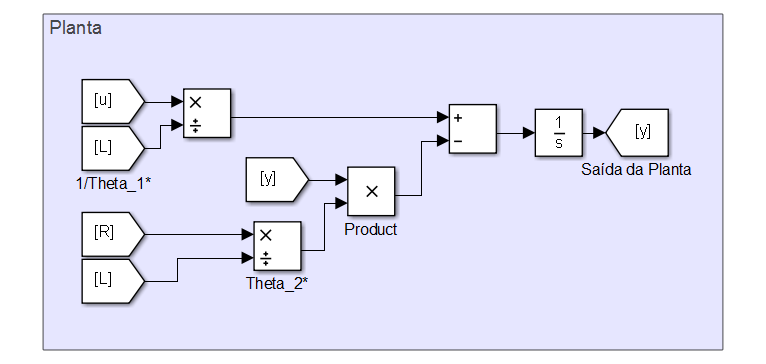
\includegraphics[width = 14 cm, height = 6 cm]{./pics/PlantaPrimeiraOrdemSemZeroPlanta.png}
\caption{Representação da equação diferencial da saída da planta de primeira ordem, $R=1.2$, $L=0.01$, $\dot{y} = 100u(t) - 120y(t)$.}
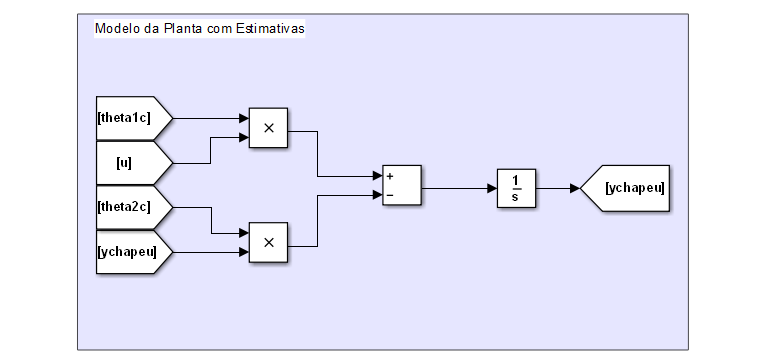
\includegraphics[width = 14 cm, height = 6 cm]{./pics/PlantaPrimeiraOrdemSemZeroModeloPlanta.png}
\caption{Representação da equação diferencial da estimativa da saída da planta de primeira ordem , $\dot{\hat{y}} = \hat{\theta_1}u(t) - \hat{\theta_2}\hat{y}(t)$}
\end{figure} 

\begin{figure}
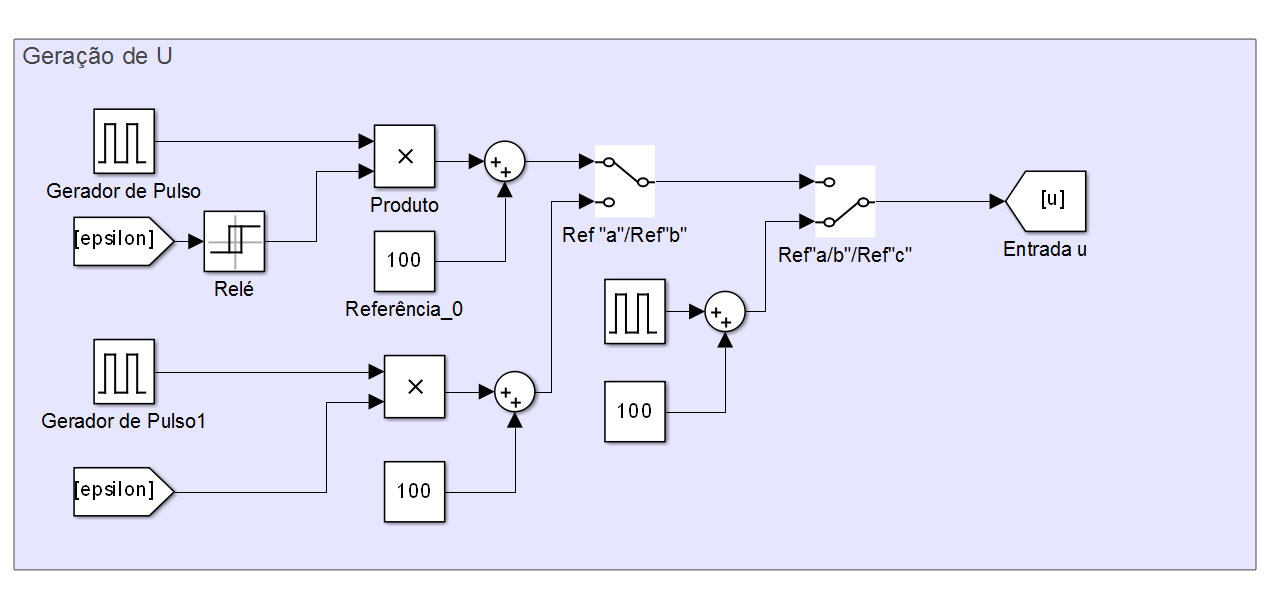
\includegraphics[width = 14 cm, height = 6 cm]{./pics/PlantaPrimeiraOrdemSemZeroU.png}
\caption{Geração do sinal de entrada u(t) para a planta de primeira ordem}
\end{figure} 

\begin{figure}
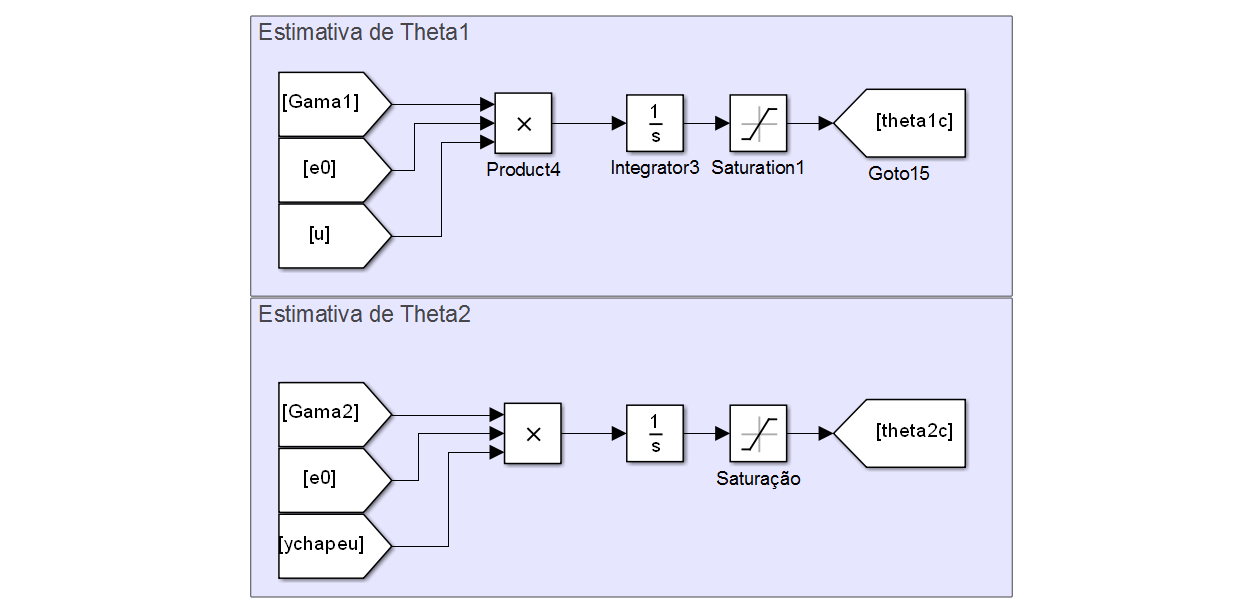
\includegraphics[width = 14 cm, height = 6 cm]{./pics/PlantaPrimeiraOrdemSemZeroEstimativas.png}
\caption{Geração e atualização das estimativas $\hat{\theta}$ para a planta de primeira ordem, $\hat{\theta_1}(0) = 80$, $\hat{\theta_2}(0) = 70$, $\gamma_1=75 $, $\gamma_2=-50$, $\hat{\theta}_1^{max}=300$, $\hat{\theta}_1^{min}=0$, $\hat{\theta}_2^{max}=500$, $\hat{\theta}_2^{min}=0$.}
\end{figure} 

\begin{figure}
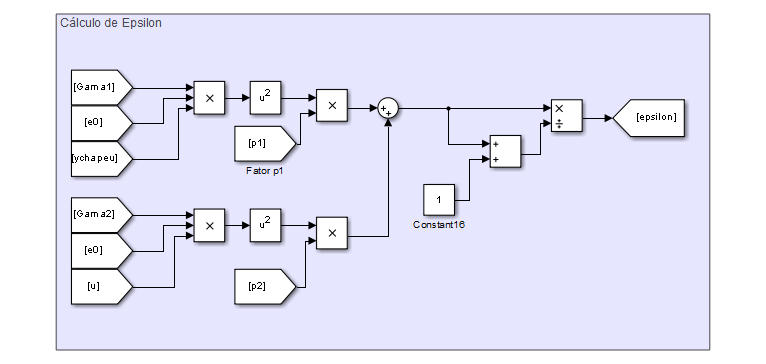
\includegraphics[width = 14 cm, height = 6 cm]{./pics/PlantaPrimeiraOrdemSemZeroEpsilon.png}
\caption{ Geração e atualização do valor de $\varepsilon$ para a planta de primeira ordem. $p_1=p_2=1/q_1^2=1/q_2^2=1/1000$.}
\end{figure} 


\subsection{Planta de Segunda Ordem com Estimador}

Observação: Pensamos nos parâmetros da planta em termos de valor absoluto, porém, na representação da EDO na forma de soma, onde $\ddot{x} = \theta_1^*u+\theta_2^*y+\theta_3*\dot{y}$, o valor do parâmetro $\theta_2^*$ e $\theta_3$ são negativos. Como representamos a EDO na forma $\ddot{x} = \theta_1^*u-\theta_2^*y-\theta_3*\dot{y}$, os ganhos $\gamma_2$ e $\gamma_3$ associados à estimativa $\hat{\theta_2}$ e $\hat{\theta_3}$ foram escolhidos negativos, de forma que os valores estimados para $\hat{\theta_2}$ e $\hat{\theta_3}$ sejam positivos.\\

Para a função de transferência $G_2(s)$, implementamos os seguintes modelos no Simulink:

\paragraph*{Comentário}
O gerador de onda quadrada tem frequência de 2Hz e amplitude de 100 unidades arbitrárias. O valor de $r_0$ é também de 100 unidades arbitrárias, assim como no teste anterior. O erro de saída $e_0$ é caracterizado da mesma forma como $y-\hat{y}$. A geração do sinal de entrada $u(t)$ é idêntica à da planta de primeira ordem.

\begin{figure}
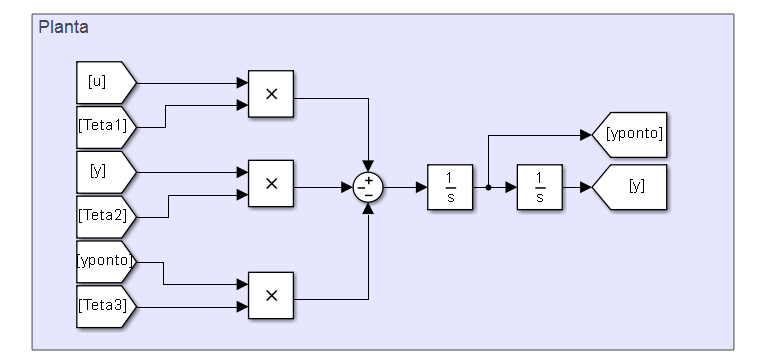
\includegraphics[width = 14 cm, height = 6 cm]{./pics/PlantaSegundaOrdemPlanta.png}
\caption{Representação da equação diferencial da saída da planta de segunda ordem,  $\ddot{y} = 39u(t) - 200y(t) - 30\dot{y}(t)$.}
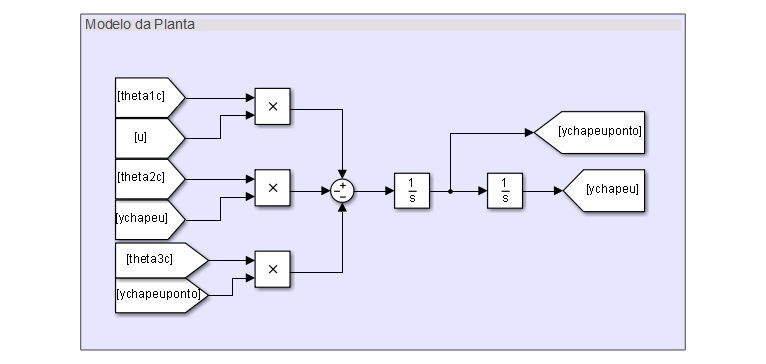
\includegraphics[width = 14 cm, height = 6 cm]{./pics/PlantaSegundaOrdemModeloPlanta.png}
\caption{Representação da equação diferencial da estimativa da saída da planta de segunda ordem , $\ddot{\hat{y}} = \hat{\theta_1}u(t) - \hat{\theta_2}\hat{y}(t) - \hat{\theta_3}\dot{\hat{y}}(t)$}
\end{figure} 

\begin{figure}
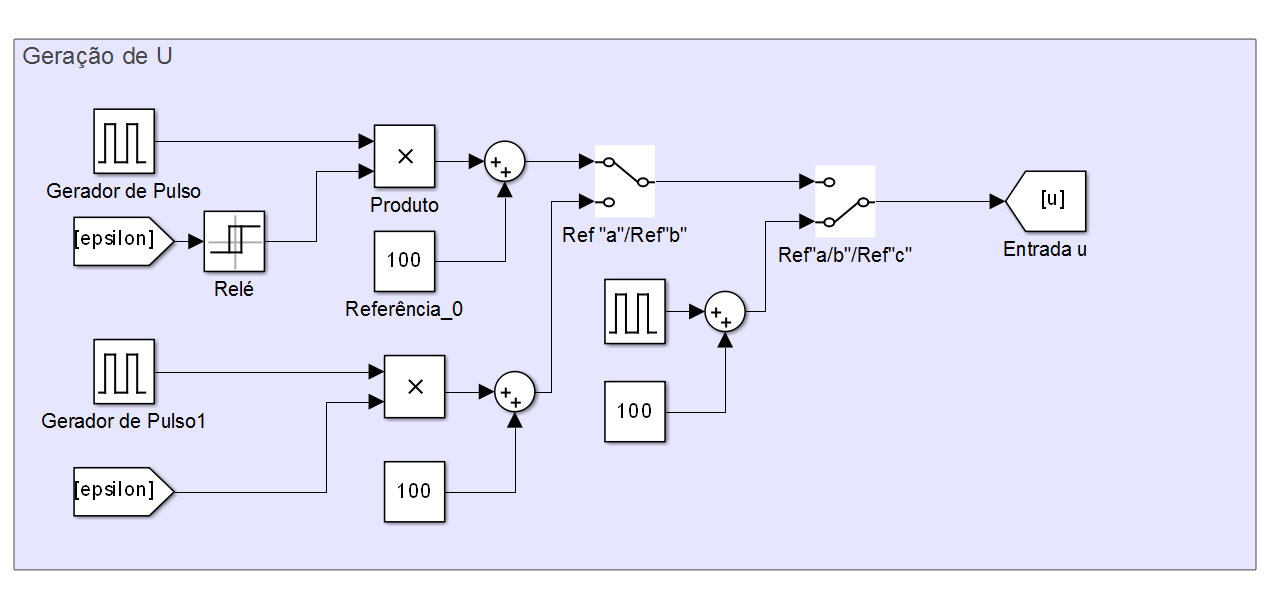
\includegraphics[width = 14 cm, height = 6 cm]{./pics/PlantaSegundaOrdemU.png}
\caption{Geração do sinal de entrada u(t) para a planta de segunda ordem}
\end{figure} 

\begin{figure}
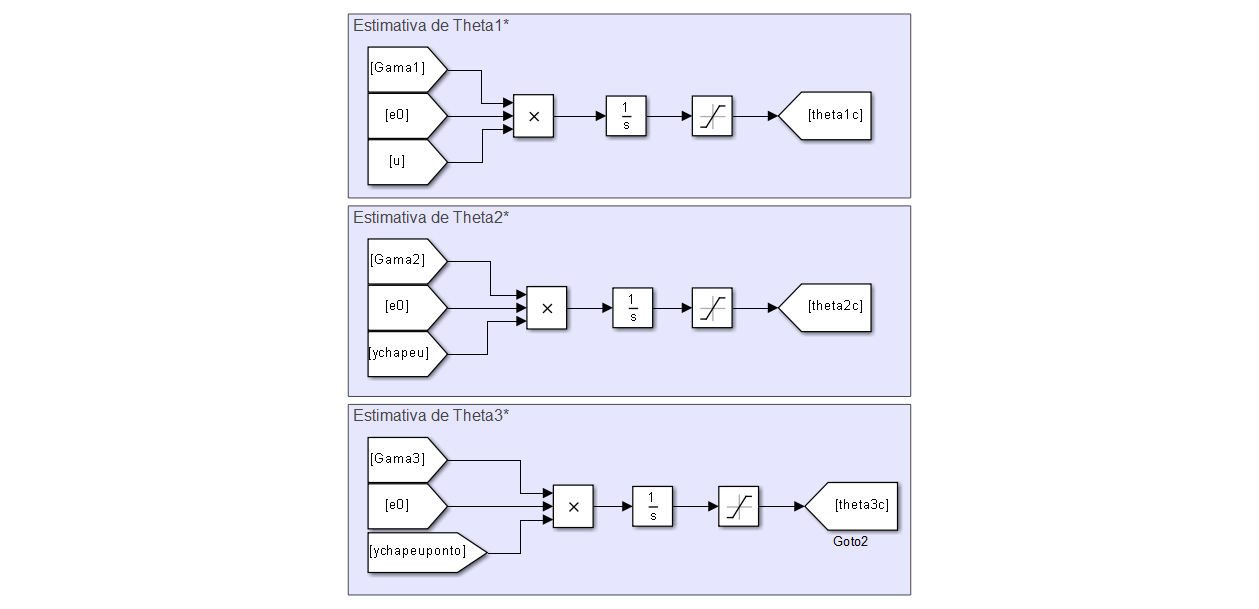
\includegraphics[width = 14 cm, height = 6 cm]{./pics/PlantaSegundaOrdemEstimativas.png}
\caption{Geração e atualização das estimativas $\hat{\theta}$ para a planta de segunda ordem, $\hat{\theta_1}(0) = 80$, $\hat{\theta_2}(0) = 70$, $\hat{\theta_3}(0) = 5$ ,  $\gamma_1=0.06 $, $\gamma_2=-0.295$,$\gamma_3=-0.035$, $\hat{\theta}_1^{max}=300000$, $\hat{\theta}_1^{min}=0$, $\hat{\theta}_2^{max}=50000$, $\hat{\theta}_2^{min}=0$, $\hat{\theta}_3^{max}=30000$, $\hat{\theta}_3^{min}=0$.}
\end{figure} 

\begin{figure}
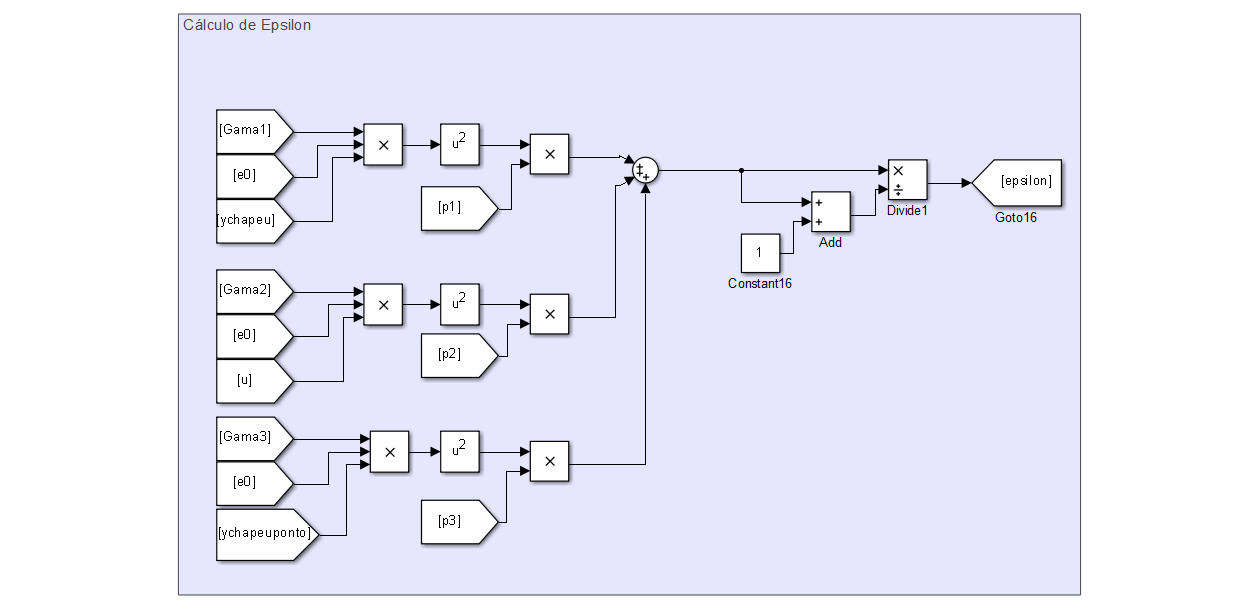
\includegraphics[width = 14 cm, height = 6 cm]{./pics/PlantaSegundaOrdemEpsilon.png}
\caption{ Geração e atualização do valor de $\varepsilon$ para a planta de segunda ordem. $p_1=p_2=p_3=1/q_1^2=1/q_2^2=1/q_3^2=10$.}
\end{figure} 


% ----------------------------------------------------------
% PARTE
% ----------------------------------------------------------
\part{Referenciais Teóricos}
% ----------------------------------------------------------

% ---
% Capitulo de revisão de literatura
% ---

Neste capítulo buscamos formalizar os conceitos e notação matemática usados enquanto indicamos referências dentro da literatura pertinente, de forma a tornar o texto auto-contido. Os conceitos a seguir são em sua maioria parafraseados do trabalho desenvolvido no livro "Robust Adaptive Control" \cite{ioannou2}.

\chapter{Modelos Estudados}

 No problema da identificação de sistemas, são necessárias várias escolhas em relação à modelagem, pois a influência de perturbações não determinísticas pode resultar em modelos que não correspondem ao comportamento do sistema em toda sua região de operação \cite{ljung}, \cite{aguirre}. Nos casos simples estudados neste trabalho, desconsideramos inicialmente a influência de perturbações não determinísticas e do atraso na medição dos dados de entrada e saída. 

 Para este trabalho, consideramos apenas a modelagem paramétrica de plantas SISO (única entrada e única saída), LTI (linear invariante no tempo), BIBO(entrada e saída limitadas) e com parâmetros concentrados que podem ser representadas no domínio da frequência através de funções de transferência \cite{chen}\cite{ogata}. Consideramos também que temos conhecimento prévio da ordem da planta, que seu grau relativo é maior ou igual a 1, que as estimativas iniciais para os parâmetros se encontram dentro de um certo alcance dos valores reais e que conhecemos o sinal de cada um destes valores. Desta forma, os modelos estudados inicialmente são da forma:
 
 \begin{align*}
 G(s) = \frac{Y(s)}{U(s)} = \frac{b_0+b_1s+b_2s^2+...+b_{n-1}s^{n-1}}{a_0+a_1s+a_2s^2+...+a_{n-1}s^{n-1}+a_ns^n}
 \end{align*} 
% ---

 onde os valores de $a_0, a_1, a_2,...,a_n,b_0,b_1,b_2,...,b_{n-1}$ estão dentro de uma determinada região e com sinal conhecido. O atraso $\Delta t$ na medição dos dados I/O é nulo e o ruído é inexistente e os sinais de entrada e saída são uniformemente limitados. 

\section{Conceitos da Literatura}

\subsection{Estimação em Tempo Real de Parâmetros}

 Dada uma estrutura de modelo para uma planta, a resposta deste modelo é determinada por certas constantes, referidas como parâmetros da planta ou do modelo. Em muitas aplicações esses parâmetros podem ser medidos ou calculados diretamente usando leis físicas ou de propriedade dos materiais (massa, resistência, volume, etc...). Em outras aplicações isto não é possível e a determinação dos parâmetros deve ser feita através da observação de seus sinais de entrada e saída. Se os parâmetros são fixos para todo o tempo t, então sua determinação se torna mais fácil, especialmente para sistemas lineares e estáveis. Nestes casos, a determinação dos parâmetros é simples através do processamento de todos os dados para um determinado período de tempo de medição (ou seja, por batelada de dados) usando técnicas desenvolvidas para o domínio da frequência ou do tempo. Estas técnicas são geralmente referidas como técnicas off-line de estimação de parâmetros ou técnicas de estimação em batelada. Em outras aplicações, a estrutura do modelo da planta pode ser conhecida, mas o valor dos parâmetros é desconhecido e muda com o tempo de acordo com condições de operação, envelhecimento do equipamento utilizado e fatores diversos. Nestes casos a estimação de parâmetros em batelada se torna inefetiva. \\

 Os esquemas apropriados de estimação a serem usados nestes casos são aqueles capazes de prover estimativas frequentes dos parâmetros do modelo da planta através do processamento dos dados de entrada e saída em tempo real, ou seja, à medida em que são coletados. Referimo-nos a estes esquemas como esquemas de estimaçao de parâmetros em tempo real \cite[p.~144-145]{ioannou2}.\\

\subsection{Sinal Rico em Frequências}

 Um sinal $u:\mathcal{R}^+\rightarrow \mathcal{R}$ é dito suficientemente rico em frequências de ordem n se contiver pelo menos n/2 frequências distintas [p.~255]\cite{ioannou2}.
 
\subsection{Sinal Estacionário} 
 
 Um sinal $u:\mathcal{R}^+\rightarrow \mathcal{R}$ é dito estacionário se a autocovariância $R_u(t,t_0)$ existe uniformemente em $t_0$ \cite[p.~256]{ioannou2}.

\subsection{Sinal Persistentemente Excitante}

 Um sinal $\phi = H(s)u $ é persistentemente excitante se e somente se $u$ é um sinal rico em frequências de ordem n e estacionário com $H(jw_1),...,H(jw_n)$ linearmente independentes em $C^n$ para todo $w_1,...,w_n \in R$ onde $w_i\neq w_k$ para $i\neq k$ \cite[p.~256-257]{ioannou2}. \\

\subsection{Método do Gradiente com Função de Custo Instantânea para uma Planta SISO, sem Normalização}
  
  
  Para um sistema qualquer as leis adaptativas podem ser implementadas sem normalização desde
  que a planta seja estável e com saída $y\in \mathcal{L}_\infty$ para entrada $u\in \mathcal{L}_\infty$. Desta forma escolhemos para este trabalho $n_s=0$, e este raciocínio pode ser feito através da justificativa para a normalização em \cite[p.~162]{ioannou2}.\\
  
 O método do gradiente ou de maior descida, introduzido na década de 60 do século 20, busca a minimização de uma função de custo $J(\theta)$ com relação a certos parâmetros ajustáveis $\theta$. Definimos o erro de saída $e_0 = y - \hat{y} = y-\theta^T\phi$, ou seja, a diferença entre a saída da planta e a saída do modelo e dado que $\phi = H(s)[u~y]^T$, onde $H(s)$ é uma matriz de funções de transferência próprias com polos estáveis. É demonstrável que $e_0$ é uma boa medida da diferença $\tilde{\theta}$ entre os valores corretos $\theta^*$ e as estimativas $\hat{\theta}$, pois um valor grande de $e_0$ implica na mesma coisa para $\tilde{\theta}$.\\
 
 Consideremos a função de custo quadrática simples $J(\theta) = {e_0}^2/2 = \frac{(y - \theta^T \phi)^2}{2}$. Para as condições estudadas, a função de custo $J$ é convexa em relação a $\theta$, o que indica a existência de um único mínimo da função. Aplicando o método do gradiente, a trajetória que minimiza $J$ é dada por $\dot{\theta} = -\Gamma \nabla J(\theta) \phi$. A partir de $J$ temos que $ \nabla J(\theta) = -e_0 \phi$ e, portanto, a lei adaptativa para o método do gradiente é dada por $\dot{\theta} = \Gamma e_0 \phi$ \cite[p.~180-186]{ioannou2}.

 
 
\subsection{Garantia de Convergência dos Parâmetros usando Função de Custo Instantânea e Regra do Gradiente Normalizada} 
 
 Para a lei adaptativa $\dot{\theta} = \Gamma \epsilon \phi$, ou algoritmo do gradiente, fica garantido que:\\
 
 \noindent $(i)$ $\epsilon,\epsilon n_s, \theta, \dot{\theta} \in \mathcal{L}_{\infty}$\\
 $(ii) \epsilon,\epsilon n_s, \theta \in \mathcal{L}_{2} $ independentemente da limitação do vetor de sinais $\phi$\\
 $(iii)$ se $n_s,\phi \in \mathcal{L}_{\infty}$ e $\phi$ é PE, então $\theta(t)$ converge exponencialmente para $\theta^*$\\
 
 Os sinais extraídos da planta contêm informações suficientes da planta para que seja obtida uma convergência das estimativas para uma região próxima aos valores corretos num tempo exponencialmente rápido desde que sejam satisfeitas as condições de persistência de excitação e limitação do sinal $\phi$\cite[p.~184-186]{ioannou2}.\\
 
 É importante notar que mesmo $\phi$ não cumprindo estas condições, o erro de saída ainda irá convergir para 0. Isto acontece pois não é necessário que o modelo da planta e a planta tenham o mesmo valor de ganho para todas as frequências, apenas para aquelas que estão sendo excitadas. Como normalmente os sinais de referência introduzidos são constantes, para um esquema de estimação qualquer, basta estimar corretamente o valor do ganho em regime permanente. \\

\subsection{Identificador de Parâmetros}

 Define-se um identificador de parâmetros como um esquema de estimador de parâmetros em tempo real que garante a convergência das estimativas dos parâmetros da planta para os valores corretos e desconhecidos dos parâmetros da planta. Esta característica adicional pode ser garantida caso o sinal introduzido tenha a característica de ser persistentemente excitante em relação ao modelo da planta\cite[p.~250-251]{ioannou2}.\\
 
 \subsection{Algoritmo do Gradiente com Projeção}
 
 Em muitos problemas práticos onde $\theta^*$ representa os parâmetros de uma planta física, é possível que tenhamos algum conhecimento à priori de onde o vetor $\theta^*$ está localizado no $\mathcal{R}^n$. Este conhecimento geralmente vem na forma de limitantes superiores e inferiores para os valores dos elementos de $\theta^*$ ou em termos de um subconjunto bem definido do $\mathcal{R}^n$. É desejável usar esta informação a respeito de $\theta^*$ no projeto de leis adaptativas que estejam limitadas a atualizar o valor de $\hat{\theta}$ na região em que $\theta^*$ está localizado. Intuitivamente, leis desta forma podem levar a tempos de convergência menores e reduzir transitórios de alta amplitude que podem ocorrer quando $\theta(0)$ é escolhido muito distante de $\theta^*$ \cite[p.~203]{ioannou2}. \\
 
 Neste trabalho, tratamos da identificação de parâmetros em plantas nas quais conhecemos os limitantes superiores e inferiores dos parâmetros, e implementamos este conhecimento na forma de saturação na saída do integrador pertinente a cada parâmetro. Desta forma, quando a tendência é que uma estimativa qualquer $\hat{\theta}_i $ irá sair da região onde $\theta^*_i$ se encontra, a estimativa deixa de atualizar até que a tendência seja de voltar ao interior da região desejada.\\
 
 \subsection{Regra de Ajuste do MIT}
 
 As leis integrativas propostas para o método do gradiente sofrem de um problema, pois é necessário gerar a derivada parcial da saída em relação às estimativas dos parâmetros $\theta$ em tempo real. Para tanto, supomos que as taxas de adaptação $\dot{\theta}$ são pequenas e que o valor das derivadas parciais de y em relação a $\theta$ e das derivadas parciais de cada derivada temporal de y em relação a $\theta$ também têm valores pequenos. A partir dessas suposições, substituímos o valor de y pelo valor da saída do modelo $\hat{y}$, e o valor de suas derivadas temporais relevantes pelo valor gerado para as derivadas de $\hat{y}$. Este método faz com que só seja possível demonstrar estabilidade local e somente em caso de $\gamma_i$ e referência pequenos. Caso contrário é possível o aparecimento do fenômeno do escape em tempo finito devido a natureza não-linear das equações impostas para as taxas de adaptação dos parâmetros. Como os valores são realimentados no modelo da planta, podemos esperar que a função de realimentação não-linear $\Phi(.)$ não tenha a origem absolutamente estável no setor [0,K], pois $\Phi(y)$ não necessariamente pertence a $\gamma(K)$  \cite{khalil}. Em contrapartida a regra de ajuste do MIT permite uma implementação relativamente simples do método do gradiente e serve a fins didáticos, nos permitindo nas simulações o uso do vetor $[u~\hat{y}]^T$ ao invés do vetor $\phi=H(s)[u~y]^T$, o qual necessita da escolha de uma matriz $H(s)$ apropriada. 
 


% ---
% ---

% ----------------------------------------------------------
% PARTE
% ----------------------------------------------------------
\part{Resultados}
% ----------------------------------------------------------
\chapter{Planta de Primeira Ordem}
% ---
\section{Sem Desligamento do Sinal PE, Referência c}

\begin{figure}
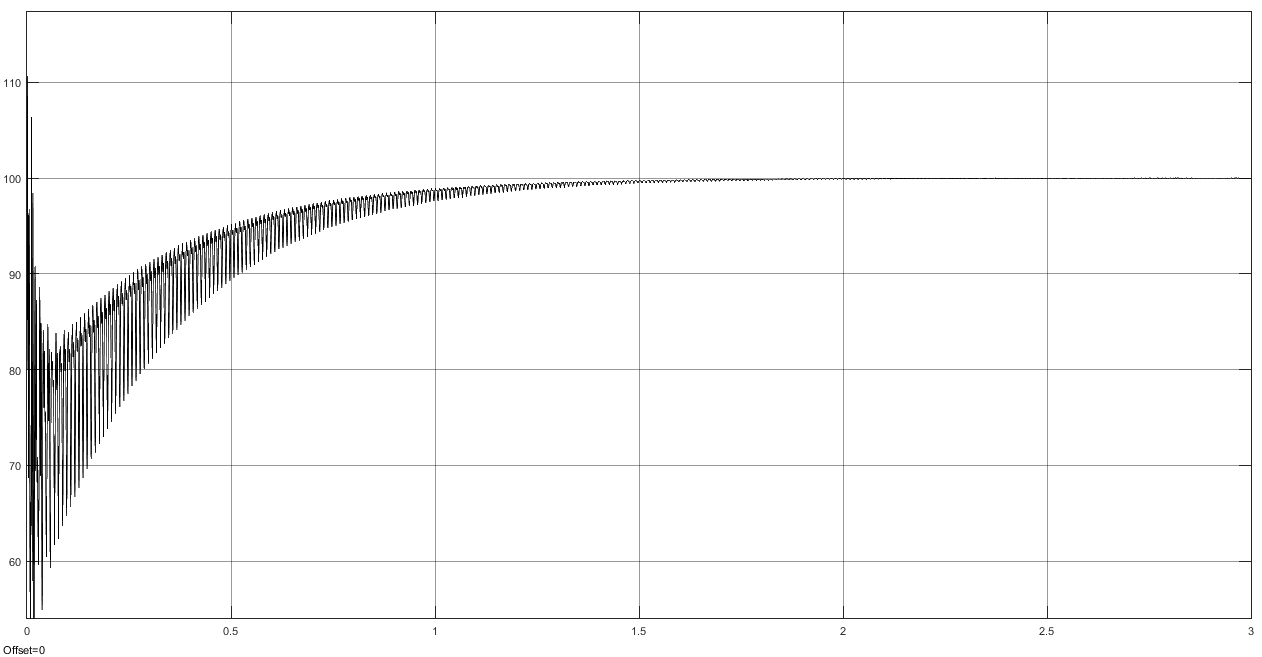
\includegraphics[width = 14 cm, height = 6 cm]{./pics/ResultadoPrimeiraOrdemEstimativaTheta1RefC.png}
\caption{Comportamento da estimativa $\hat{\theta_1}$ para a planta de primeira ordem no tempo entre 0 e 3 segundos para a referência c}
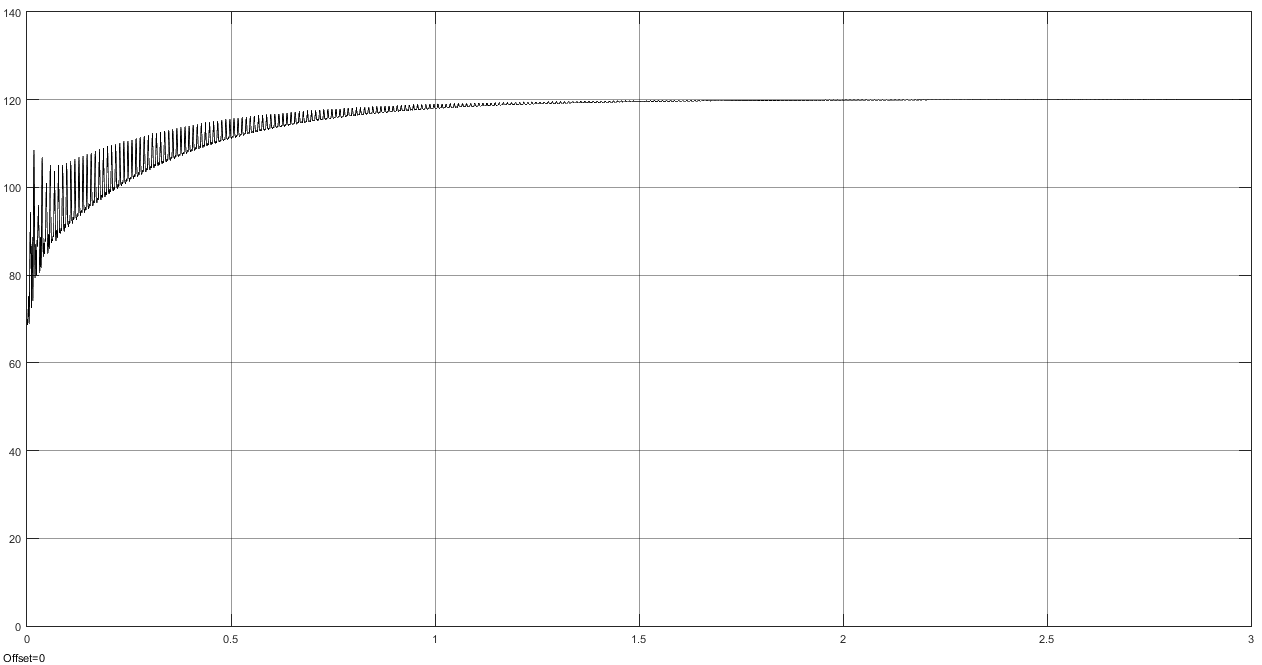
\includegraphics[width = 14 cm, height = 6 cm]{./pics/ResultadoPrimeiraOrdemEstimativaTheta2RefC.png}
\caption{Comportamento da estimativa $\hat{\theta_2}$ para a planta de primeira ordem no tempo entre 0 e 3 segundos para a referência c}
\end{figure}
\begin{figure}
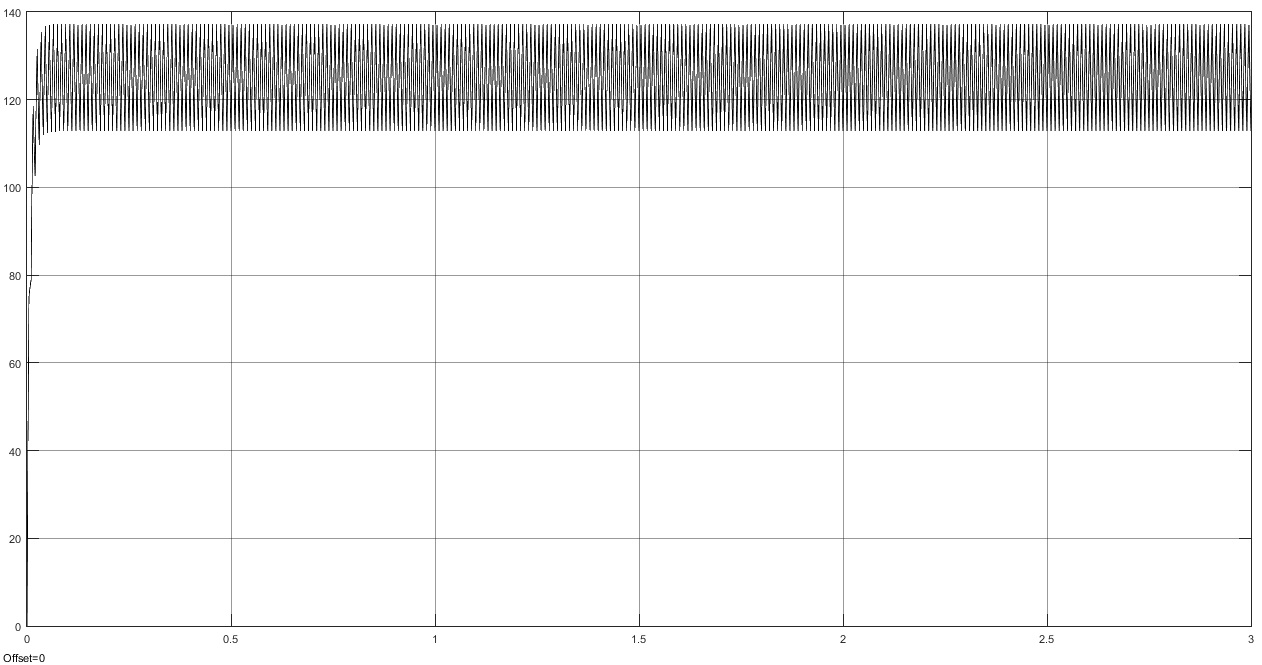
\includegraphics[width = 14 cm, height = 6 cm]{./pics/ResultadoPrimeiraOrdemEstimativaYRefC.png}
\caption{Comportamento da saída da planta de primeira ordem no tempo entre 0 e 3 segundos para a referência c}
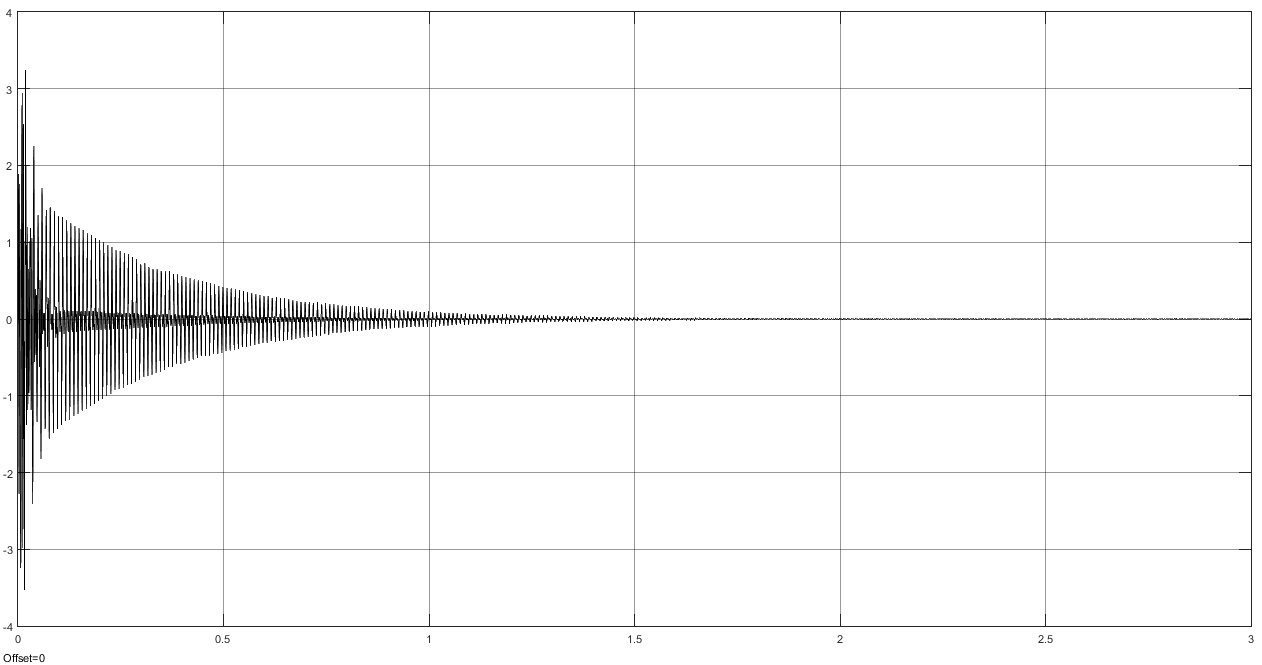
\includegraphics[width = 14 cm, height = 6 cm]{./pics/ResultadoPrimeiraOrdemEstimativaE0RefC.png}
\caption{Erro de saída da planta de primeira ordem no tempo entre 0 e 3 segundos para a referência c}
\end{figure} 

Para uma referência "c" que é PE em relação à planta de primeira ordem $\forall t$, conseguimos a convergência dos parâmetros para seus valores verdadeiros, $\hat{\theta_1}=\theta_1^*=100$, $\hat{\theta_2} = \theta_2^* = 120$,  dentro de 2 segundos de simulação(Figuras 11 e 12), porém ao custo de introduzir um sinal que torna o valor de saída y da planta oscilante para todo t (Figura 13). Vemos também que o comportamento do modelo da planta converge para o desejado, pois o erro de saída $e_0 = y - \hat{y}$ tende a 0 (Figura 14).\\

\section{Com Desligamento do Sinal PE, Referência b}


\begin{figure}
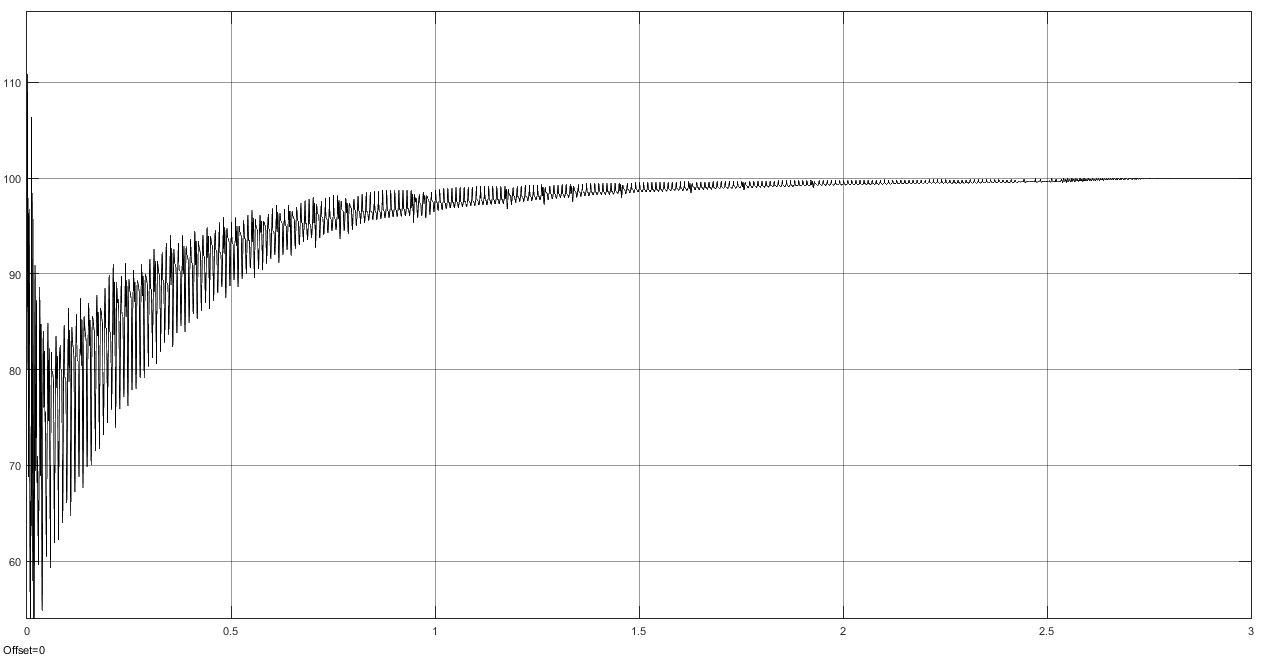
\includegraphics[width = 14 cm, height = 6 cm]{./pics/ResultadoPrimeiraOrdemEstimativaTheta1RefB.png}
\caption{Comportamento da estimativa $\hat{\theta_1}$ para a planta de primeira ordem no tempo entre 0 e 3 segundos para a referência b}
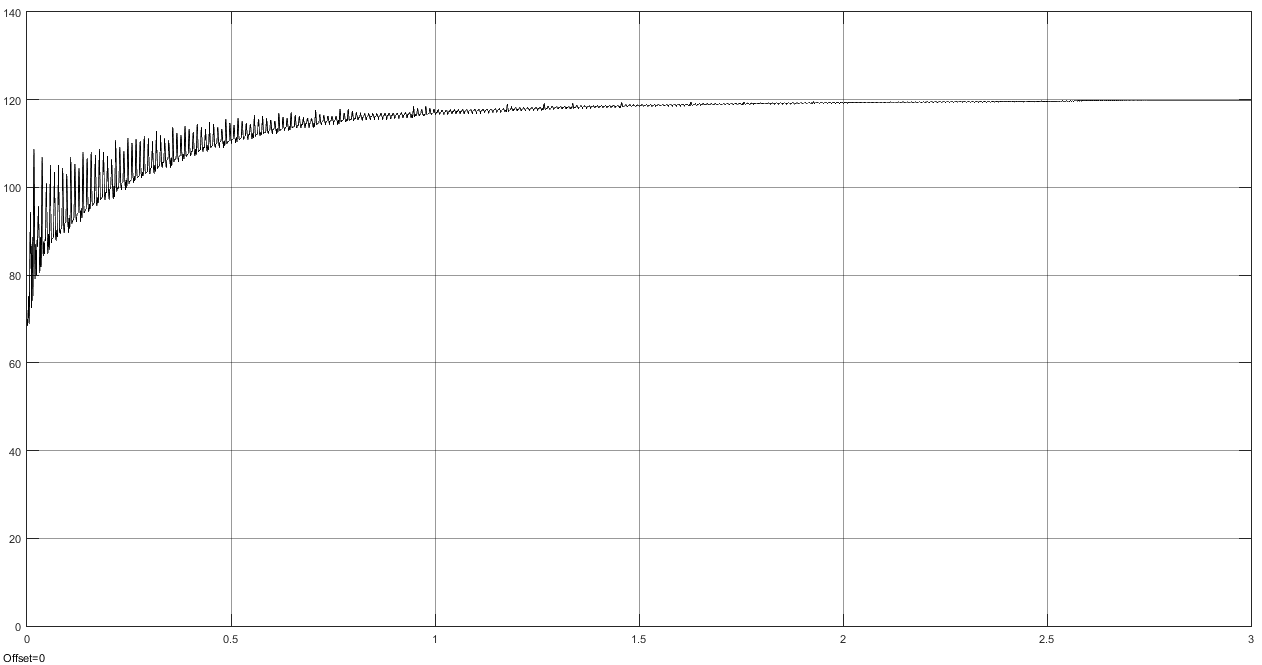
\includegraphics[width = 14 cm, height = 6 cm]{./pics/ResultadoPrimeiraOrdemEstimativaTheta2RefB.png}
\caption{Comportamento da estimativa $\hat{\theta_2}$ para a planta de primeira ordem no tempo entre 0 e 3 segundos para a referência b}
\end{figure}
\begin{figure}
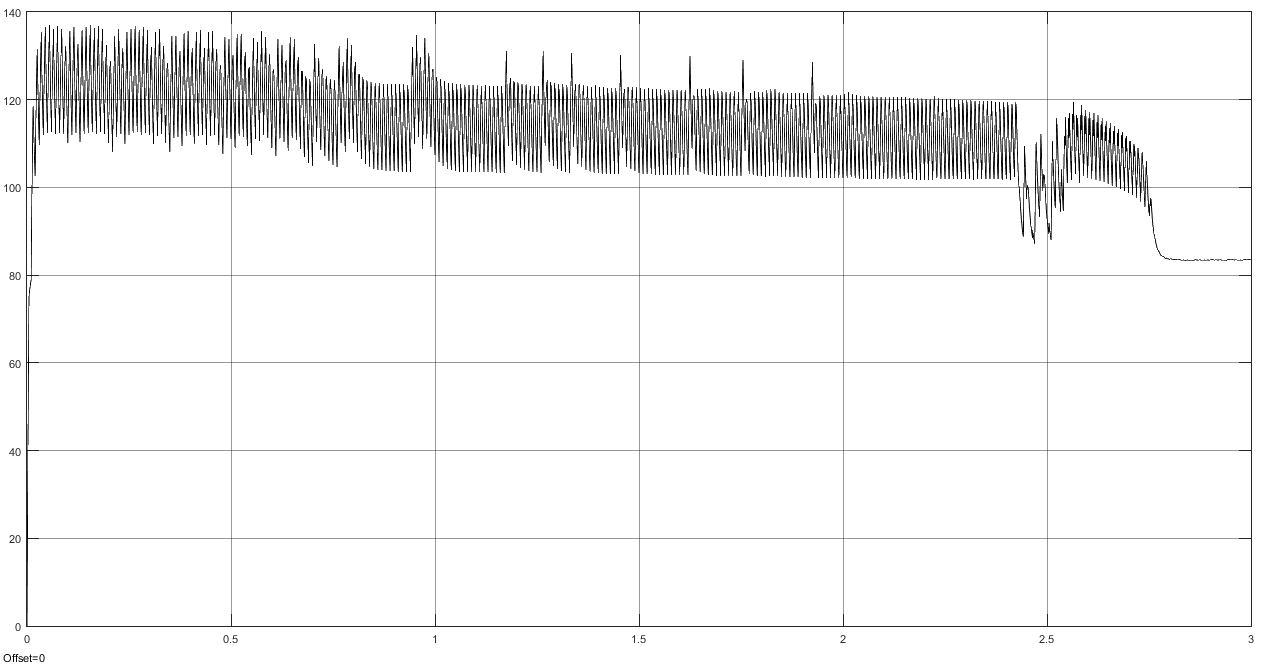
\includegraphics[width = 14 cm, height = 6 cm]{./pics/ResultadoPrimeiraOrdemEstimativaYRefB.png}
\caption{Comportamento da saída da planta de primeira ordem no tempo entre 0 e 3 segundos para a referência b}
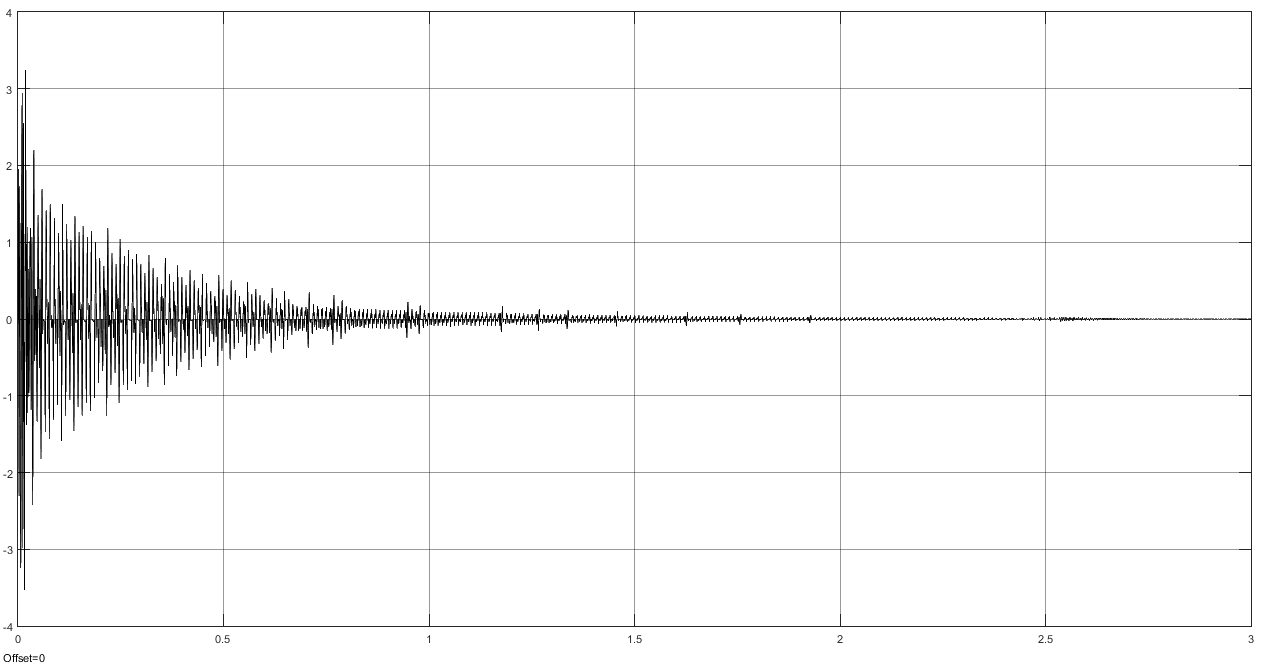
\includegraphics[width = 14 cm, height = 6 cm]{./pics/ResultadoPrimeiraOrdemEstimativaE0RefB.png}
\caption{Erro de saída da planta de primeira ordem no tempo entre 0 e 3 segundos para a referência b}
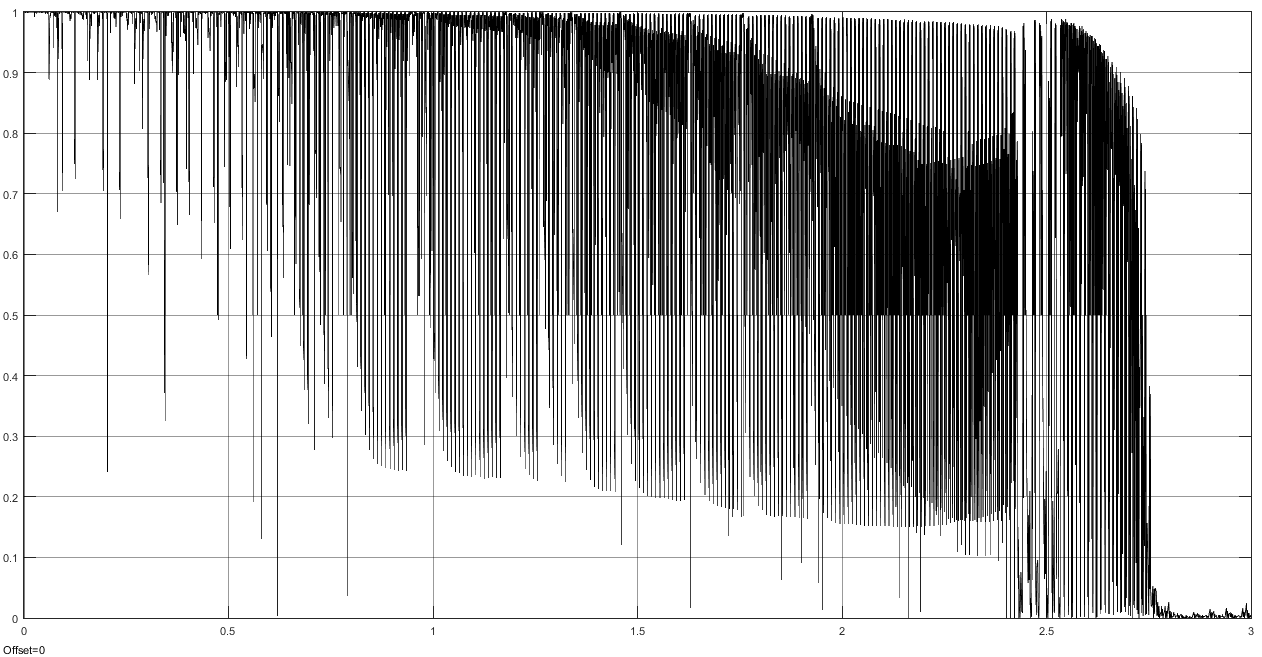
\includegraphics[width = 14 cm, height = 6 cm]{./pics/ResultadoPrimeiraOrdemEstimativaEpsilonRefB.png}
\caption{Comportamento da figura de mérito $\varepsilon$ para planta de primeira ordem no tempo entre 0 e 3 segundos para a referência b}
\end{figure}

Neste caso ainda conseguimos atingir a convergência dos parâmetros para seus valores verdadeiros, $\hat{\theta_1}=\theta_1^*=100$, $\hat{\theta_2} = \theta_2^* = 120$ (Figuras 15 e 16), porém a saída da planta só é oscilante para um duração de tempo finita(Figura 17). O comportamento do modelo da planta converge, pois o erro de saída tende a 0 (Figura 18), e a parte PE do sinal de referência "b" desliga pois $\varepsilon$ tende a 0 (Figura 19).\\

\section{Com Desligamento do Sinal PE, Referência a}
% segundo capitulo de Resultados

\begin{figure}
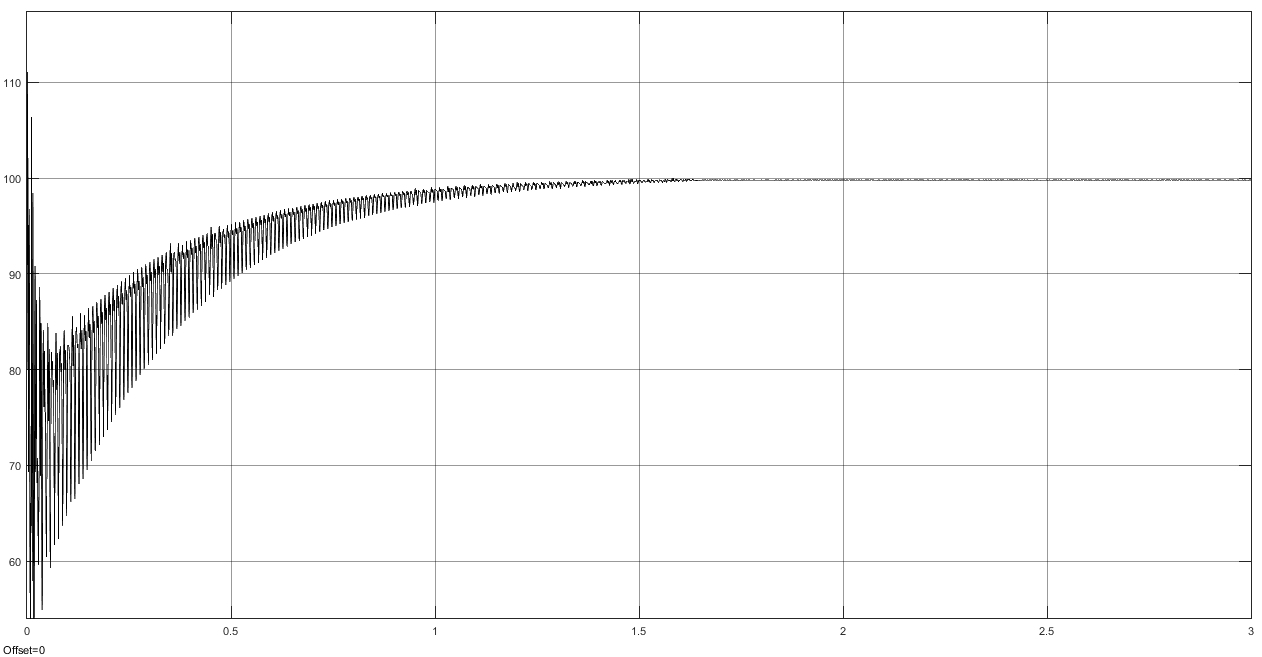
\includegraphics[width = 14 cm, height = 6 cm]{./pics/ResultadoPrimeiraOrdemEstimativaTheta1RefA.png}
\caption{Comportamento da estimativa $\hat{\theta_1}$ para a planta de primeira ordem no tempo entre 0 e 3 segundos para a referência a}
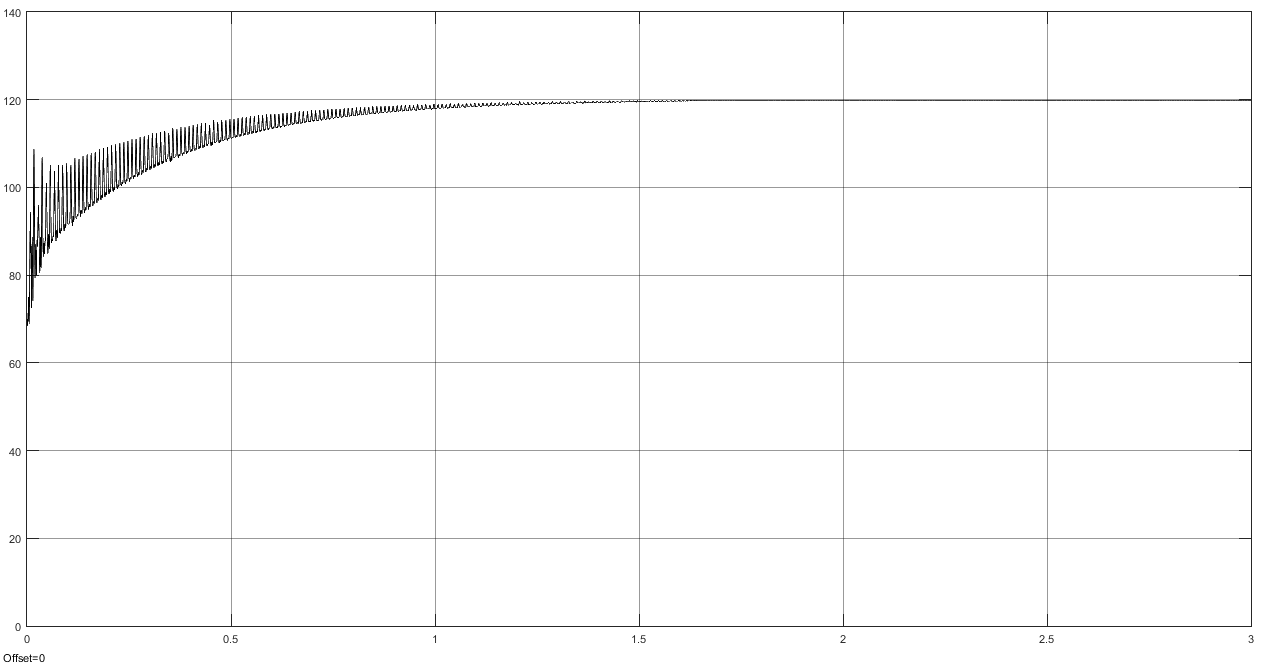
\includegraphics[width = 14 cm, height = 6 cm]{./pics/ResultadoPrimeiraOrdemEstimativaTheta2RefA.png}
\caption{Comportamento da estimativa $\hat{\theta_2}$ para a planta de primeira ordem no tempo entre 0 e 3 segundos para a referência a}
\end{figure}
\begin{figure}
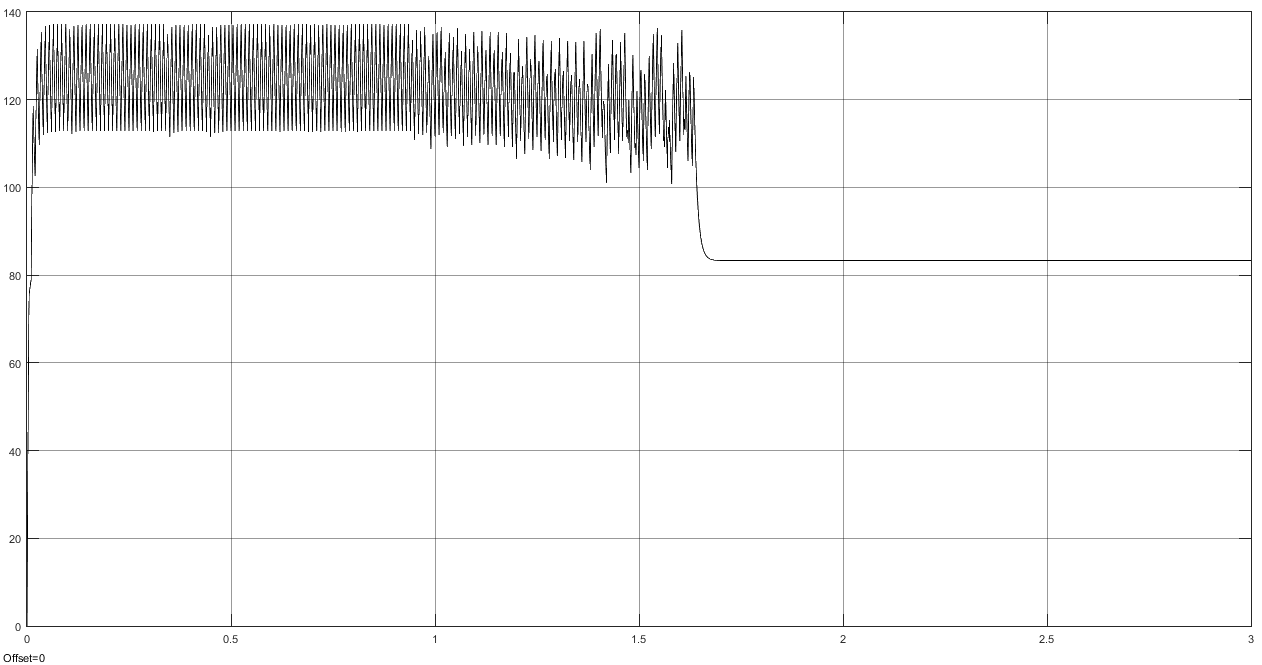
\includegraphics[width = 14 cm, height = 6 cm]{./pics/ResultadoPrimeiraOrdemEstimativaYRefA.png}
\caption{Comportamento da saída da planta de primeira ordem no tempo entre 0 e 3 segundos para a referência a}
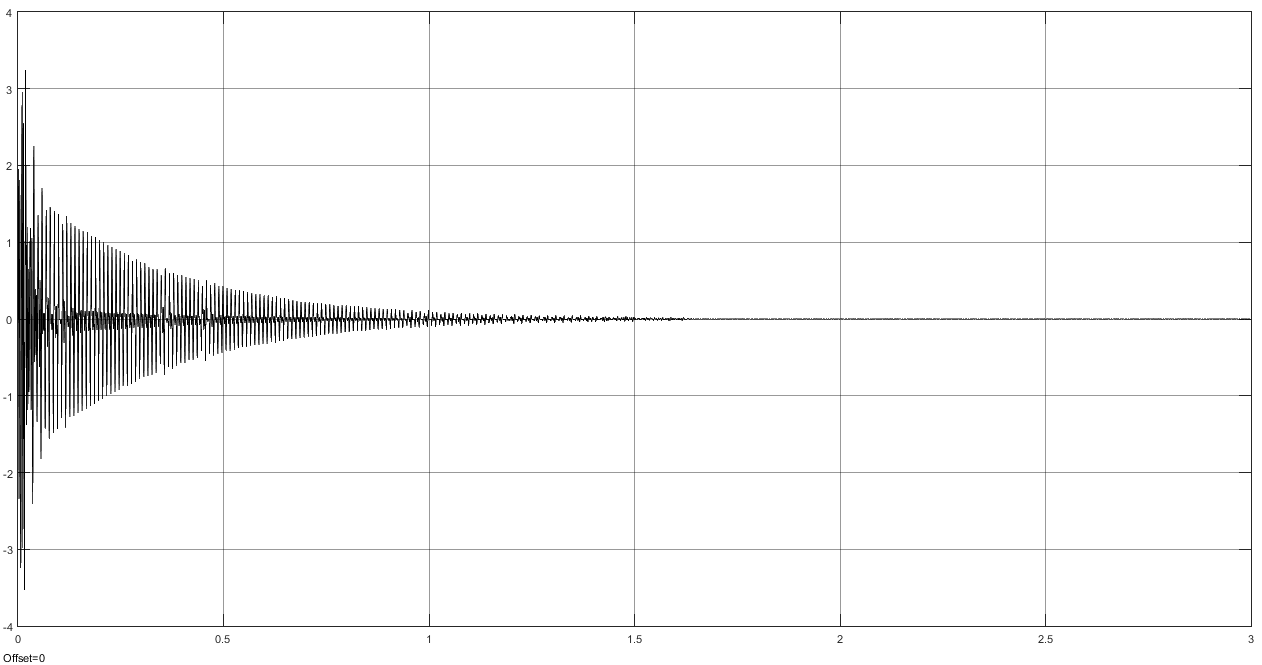
\includegraphics[width = 14 cm, height = 6 cm]{./pics/ResultadoPrimeiraOrdemEstimativaE0RefA.png}
\caption{Erro de saída da planta de primeira ordem no tempo entre 0 e 3 segundos para a referência a}
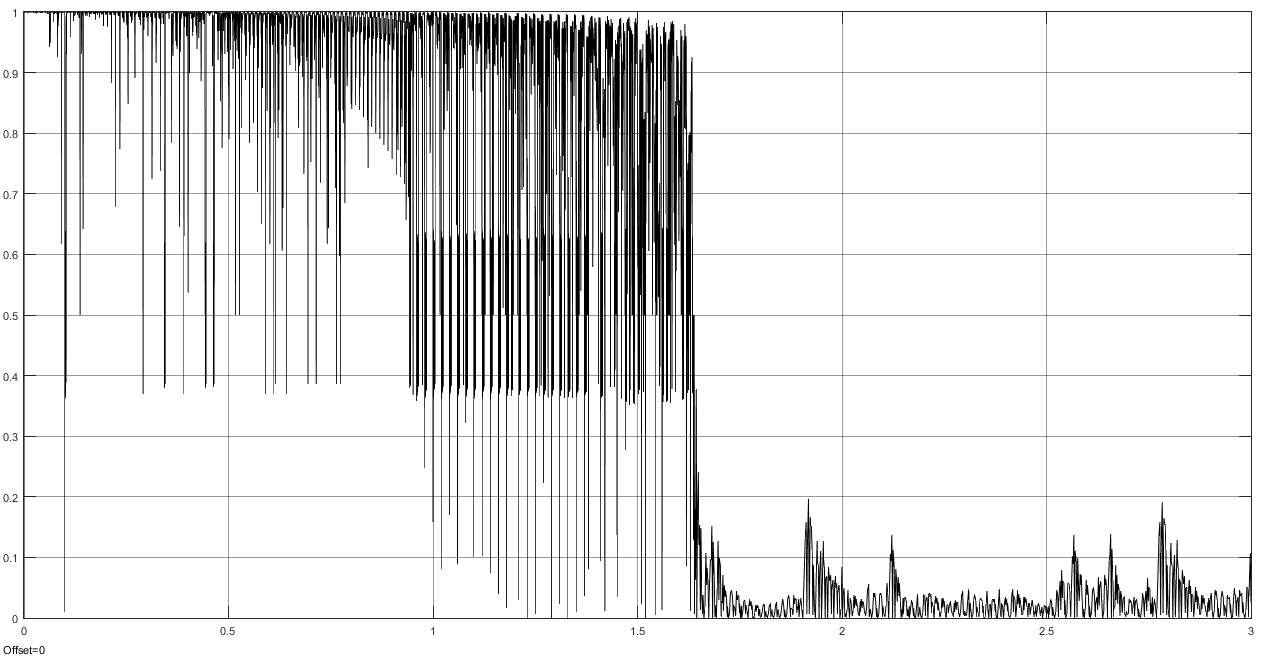
\includegraphics[width = 14 cm, height = 6 cm]{./pics/ResultadoPrimeiraOrdemEstimativaEpsilonRefA.png}
\caption{Comportamento da figura de mérito $\varepsilon$ para a planta de primeira ordem no tempo entre 0 e 3 segundos para a referência a}
\end{figure}

Neste caso, com o uso de um relé com amplitude igual a 0.5, conseguimos um resultado similar ao da referência b. A convergência dos parâmetros para os valores verdadeiros $\hat{\theta_1}=\theta_1^*=100$, $\hat{\theta_2} = \theta_2^* = 120$ acontece (Figuras 19 e 20). A saída da planta só é oscilante durante um tempo finito e menor que no caso da referência b (Figura 21). O comportamento do modelo da planta converge pois o erro de saída tende a 0(Figura 22), e a parte PE do sinal desliga pois $\varepsilon$ se mantém em um valor consistentemente menor que a amplitude do relé após a adaptação(Figura 23). Podemos comparar o desempenho para cada referência através da Tabela 1 para o tempo de convergência e da Tabela 2 para a precisão.\\



% ---
\chapter{Planta de Segunda Ordem}
% -----


\section{Sem Desligamento do Sinal PE, Referência c}

\begin{figure}
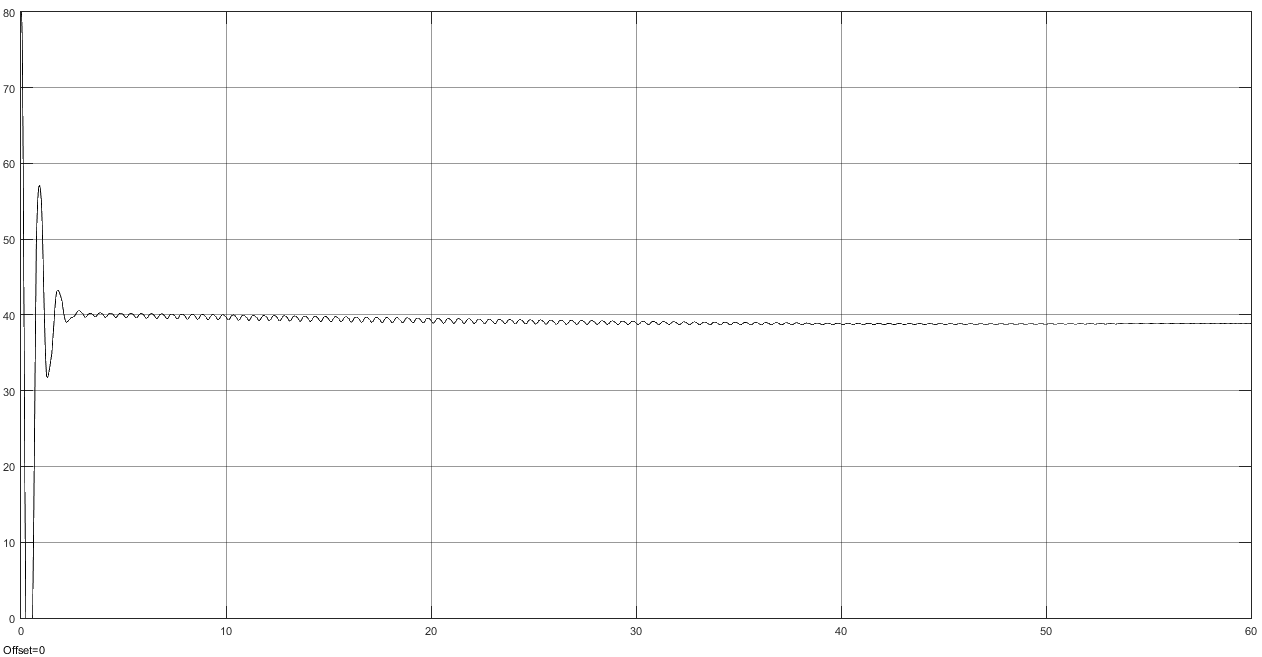
\includegraphics[width = 14 cm, height = 6 cm]{./pics/ResultadoSegundaOrdemEstimativaTheta1RefC.png}
\caption{Comportamento da estimativa $\hat{\theta_1}$ para a planta de segunda ordem no tempo entre 0 e 60 segundos para a referência c}
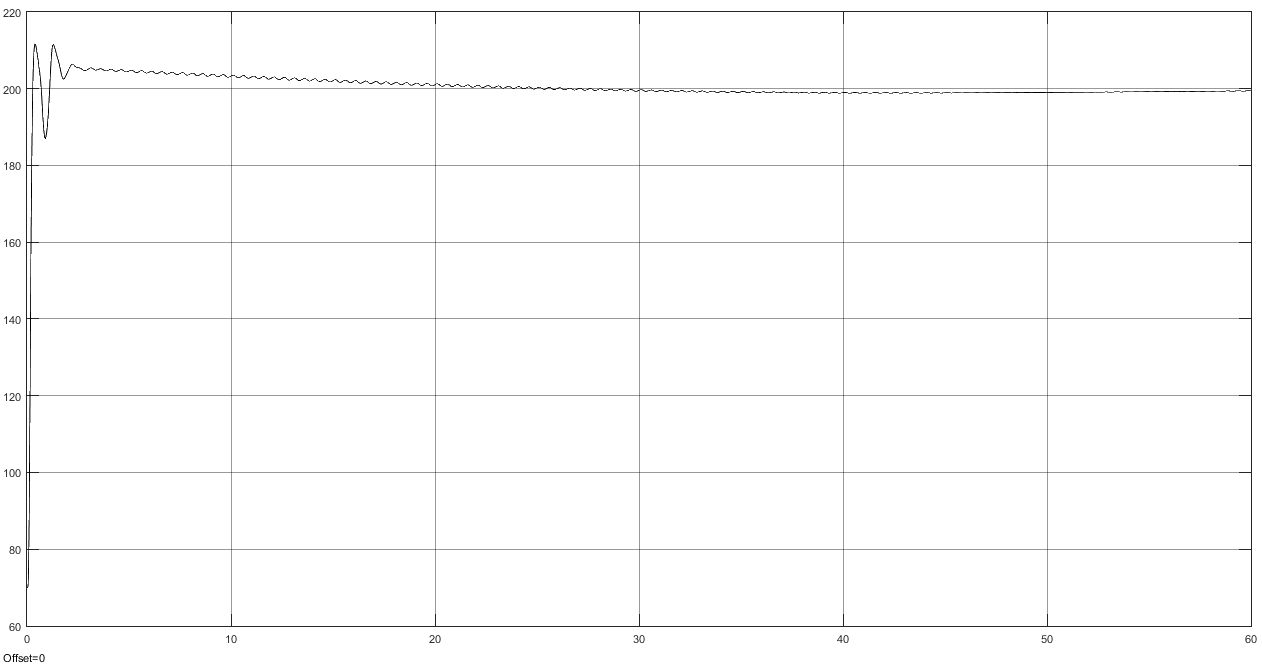
\includegraphics[width = 14 cm, height = 6 cm]{./pics/ResultadoSegundaOrdemEstimativaTheta2RefC.png}
\caption{Comportamento da estimativa $\hat{\theta_2}$ para a planta de segunda ordem no tempo entre 0 e 60 segundos para a referência c}
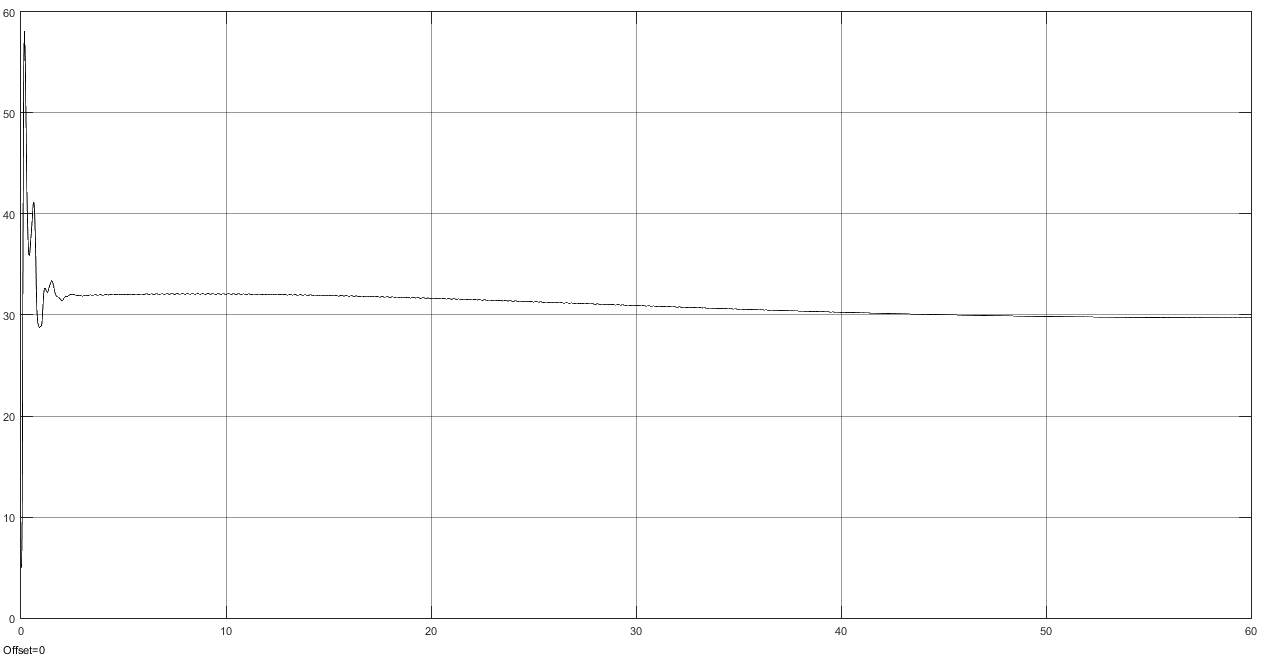
\includegraphics[width = 14 cm, height = 6 cm]{./pics/ResultadoSegundaOrdemEstimativaTheta3RefC.png}
\caption{Comportamento da estimativa $\hat{\theta_3}$ para a planta de segunda ordem no tempo entre 0 e 60 segundos para a referência c}
\end{figure}
\begin{figure}
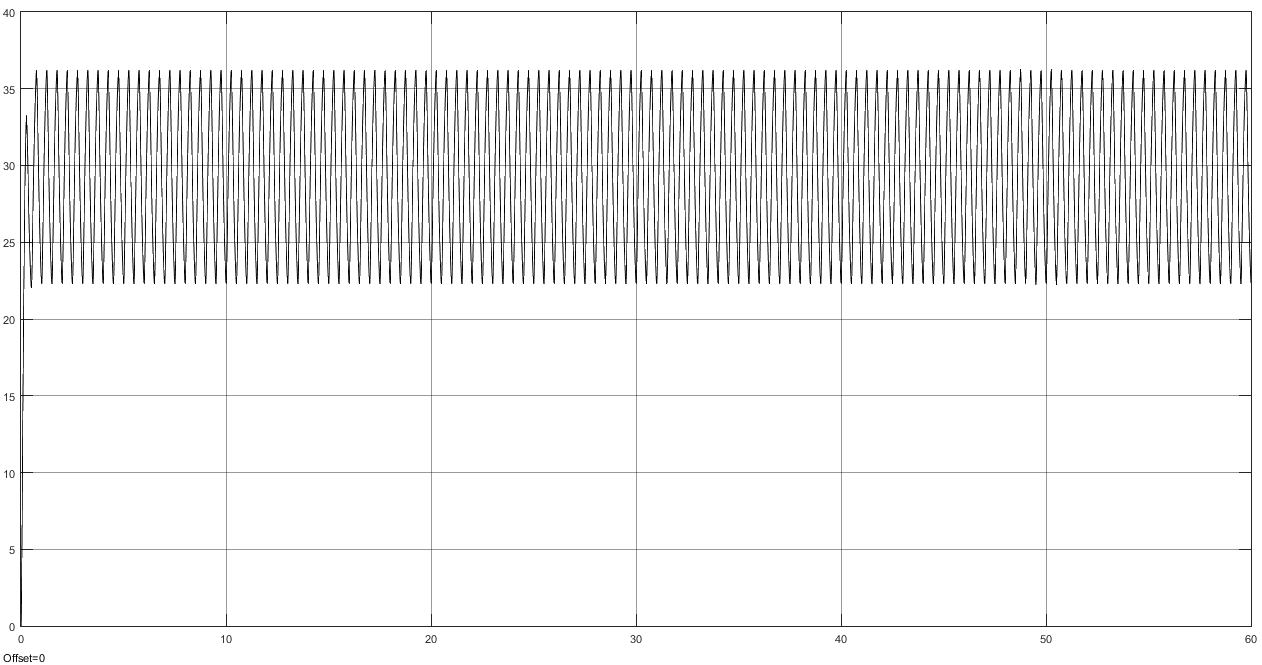
\includegraphics[width = 14 cm, height = 6 cm]{./pics/ResultadoSegundaOrdemEstimativaYRefC.png}
\caption{Comportamento da saída da planta de segunda ordem no tempo entre 0 e 60 segundos para a referência c}
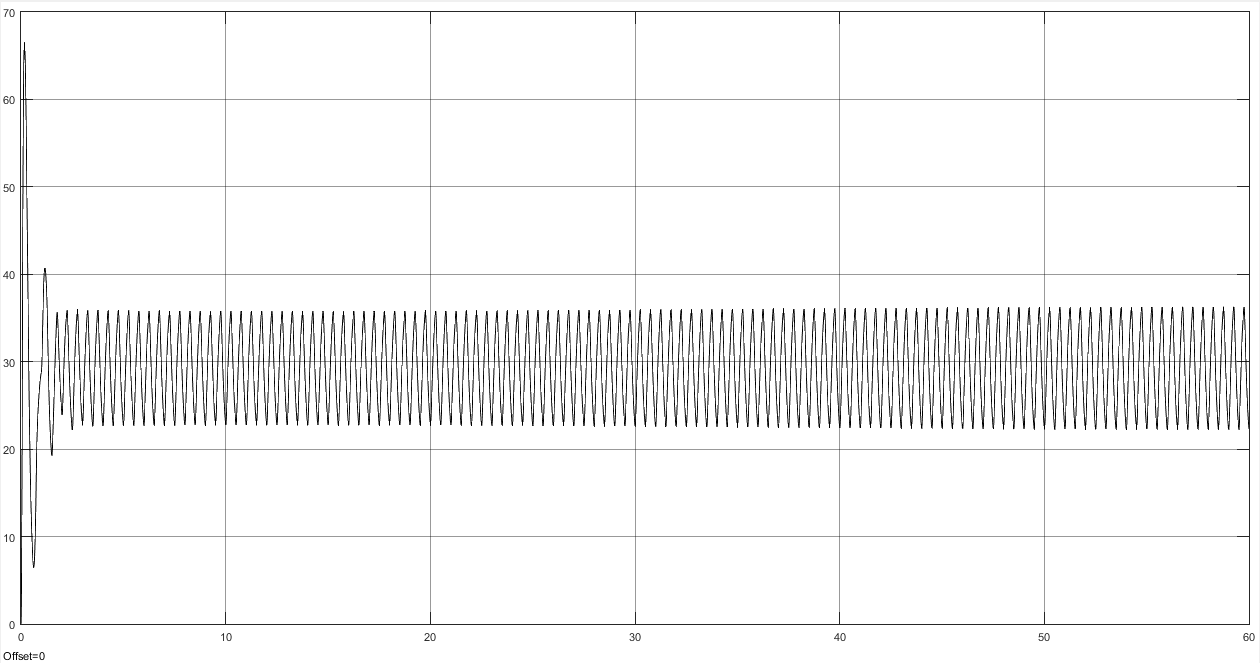
\includegraphics[width = 14 cm, height = 6 cm]{./pics/ResultadoSegundaOrdemEstimativaYcRefC.png}
\caption{Comportamento da saída do modelo da planta de segunda ordem no tempo entre 0 e 60 segundos para a referência c}
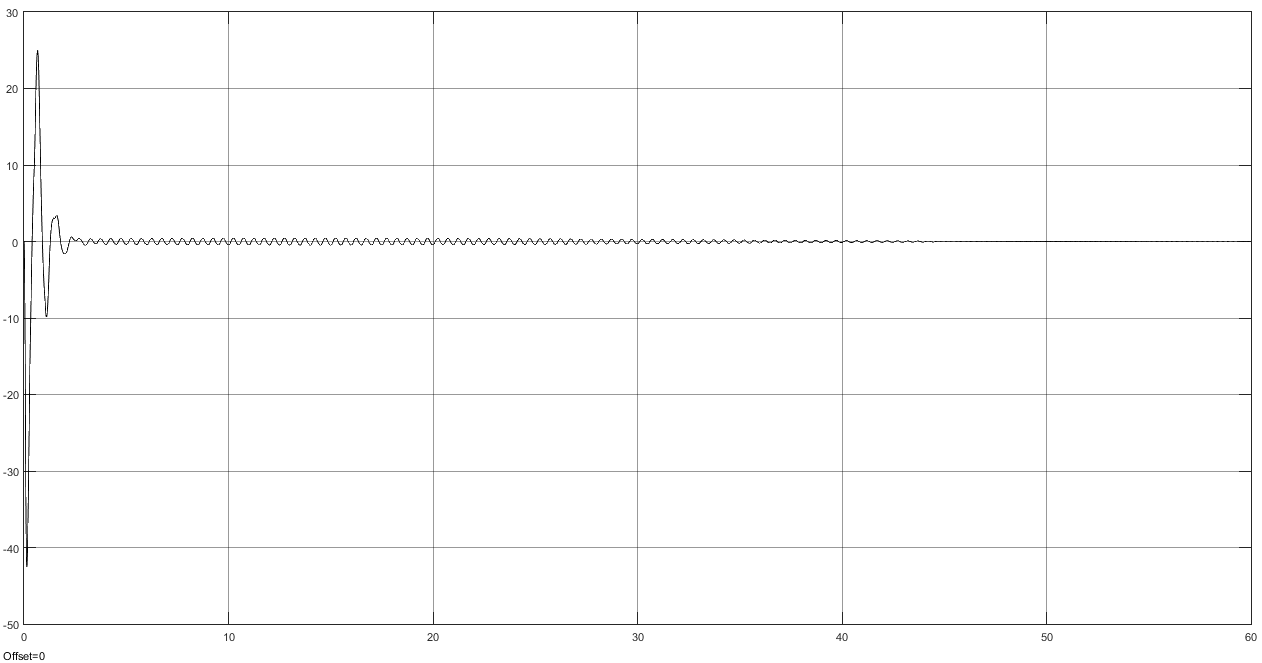
\includegraphics[width = 14 cm, height = 6 cm]{./pics/ResultadoSegundaOrdemEstimativaE0RefC.png}
\caption{Erro de saída da planta de segunda ordem no tempo entre 0 e 60 segundos para a referência c}
\end{figure} 


Para uma referência persistentemente excitante em relação à planta de segunda ordem, conseguimos a convergência dos parâmetros para seus valores verdadeiros,$\hat{\theta_1}=\theta_1^*=39$, $\hat{\theta_2} = \theta_2^* = 200$, $\hat{\theta_3} = \theta_2^* = 30$, dentro de 60 segundos de simulação (Figuras 24-26), porém ao custo de introduzir um sinal que torna o valor de saída da planta oscilante para todo t(Figura 27). Para este modelo é possível observar diferenças no comportamento do modelo da planta e a planta real, comparando as Figuras 27 e 28, porém eventualmente o modelo da planta converge pois o erro de saída tende a 0(Figura 29).\\

\section{Com Desligamento do Sinal PE, Referência b}


\begin{figure}
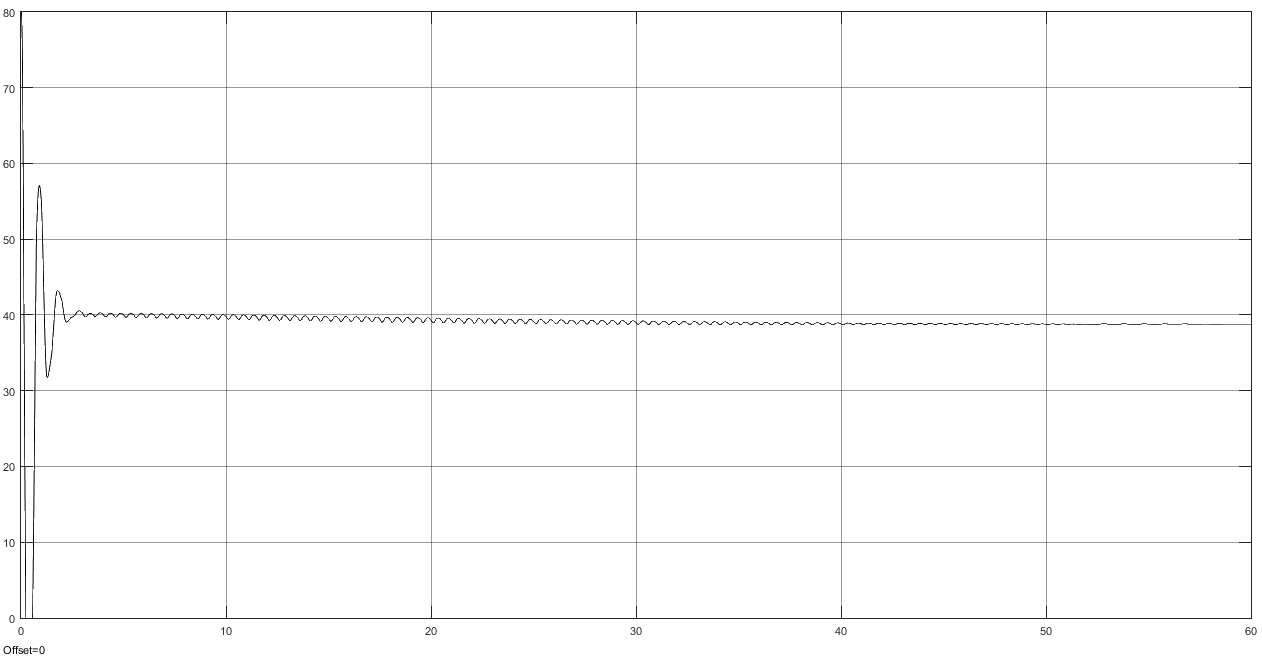
\includegraphics[width = 14 cm, height = 6 cm]{./pics/ResultadoSegundaOrdemEstimativaTheta1RefB.png}
\caption{Comportamento da estimativa $\hat{\theta_1}$ para a planta de segunda ordem no tempo entre 0 e 60 segundos para a referência b}
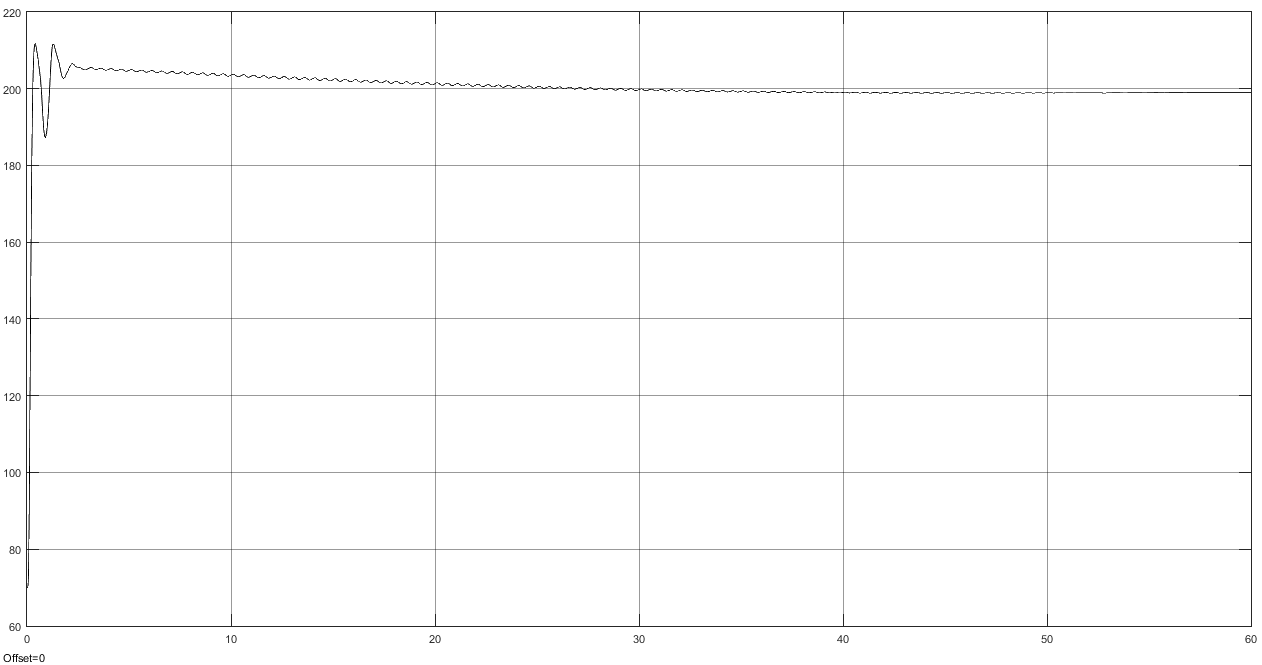
\includegraphics[width = 14 cm, height = 6 cm]{./pics/ResultadoSegundaOrdemEstimativaTheta2RefB.png}
\caption{Comportamento da estimativa $\hat{\theta_2}$ para a planta de segunda ordem no tempo entre 0 e 60 segundos para a referência b}
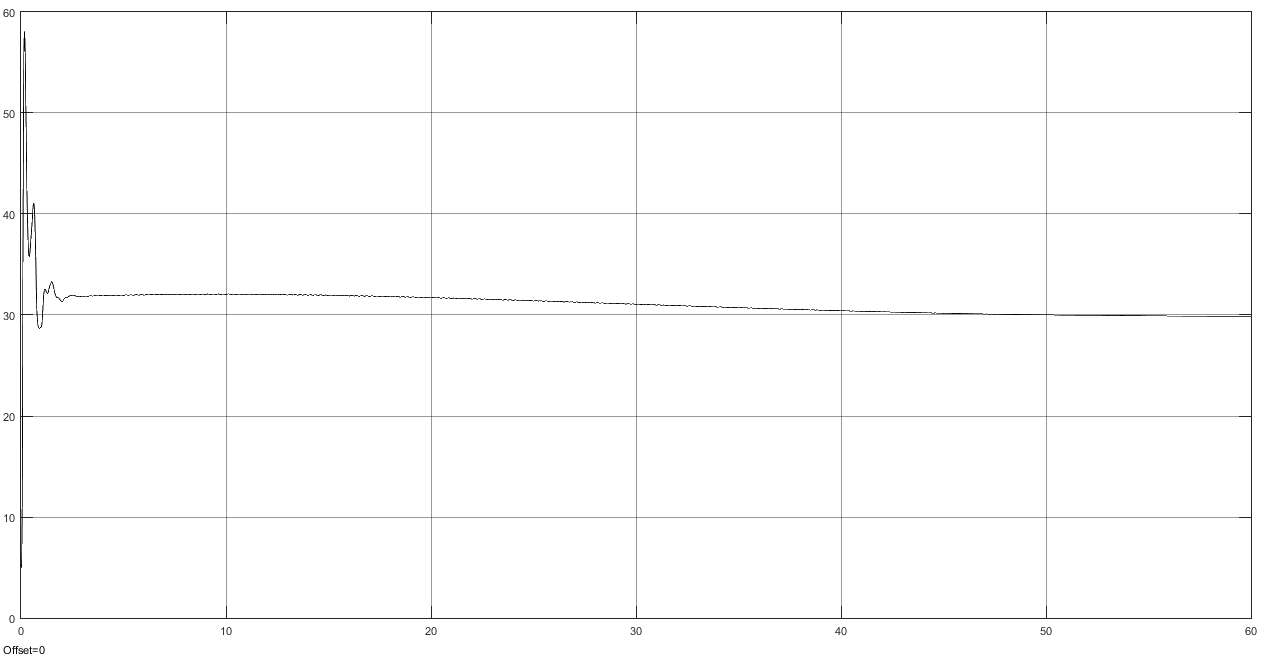
\includegraphics[width = 14 cm, height = 6 cm]{./pics/ResultadoSegundaOrdemEstimativaTheta3RefB.png}
\caption{Comportamento da estimativa $\hat{\theta_3}$ para a planta de segunda ordem no tempo entre 0 e 60 segundos para a referência b}
\end{figure}
\begin{figure}
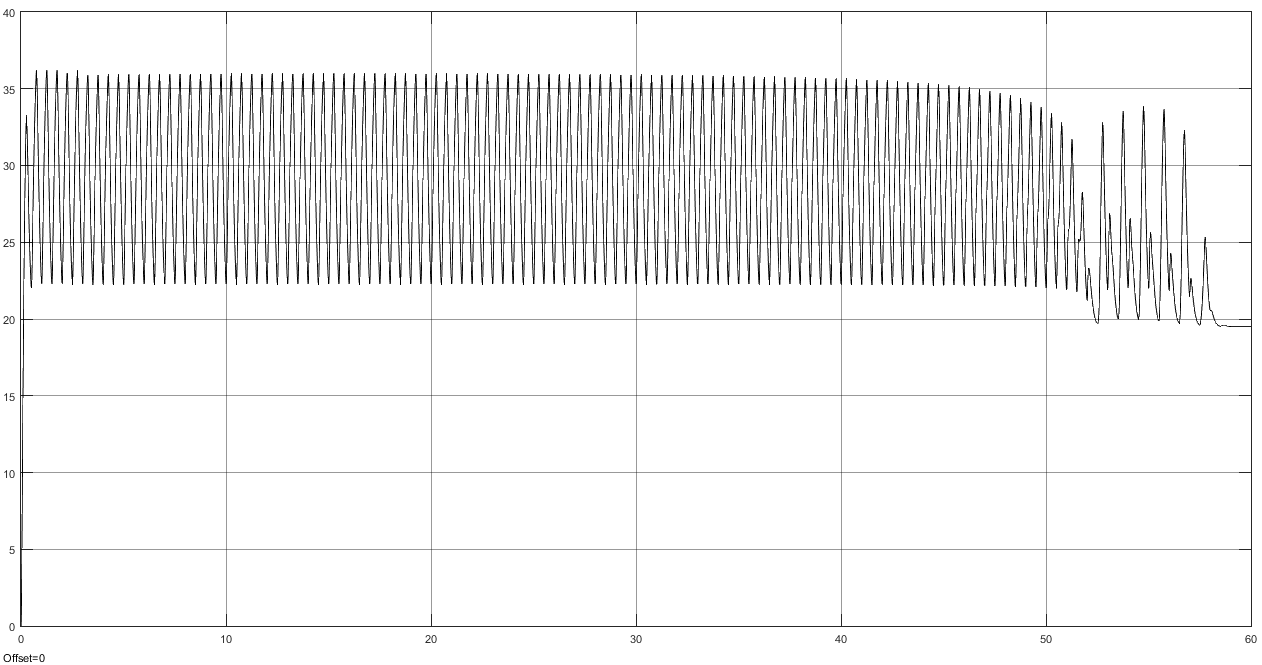
\includegraphics[width = 14 cm, height = 6 cm]{./pics/ResultadoSegundaOrdemEstimativaYRefB.png}
\caption{Comportamento da saída da planta de segunda ordem no tempo entre 0 e 60 segundos para a referência b}
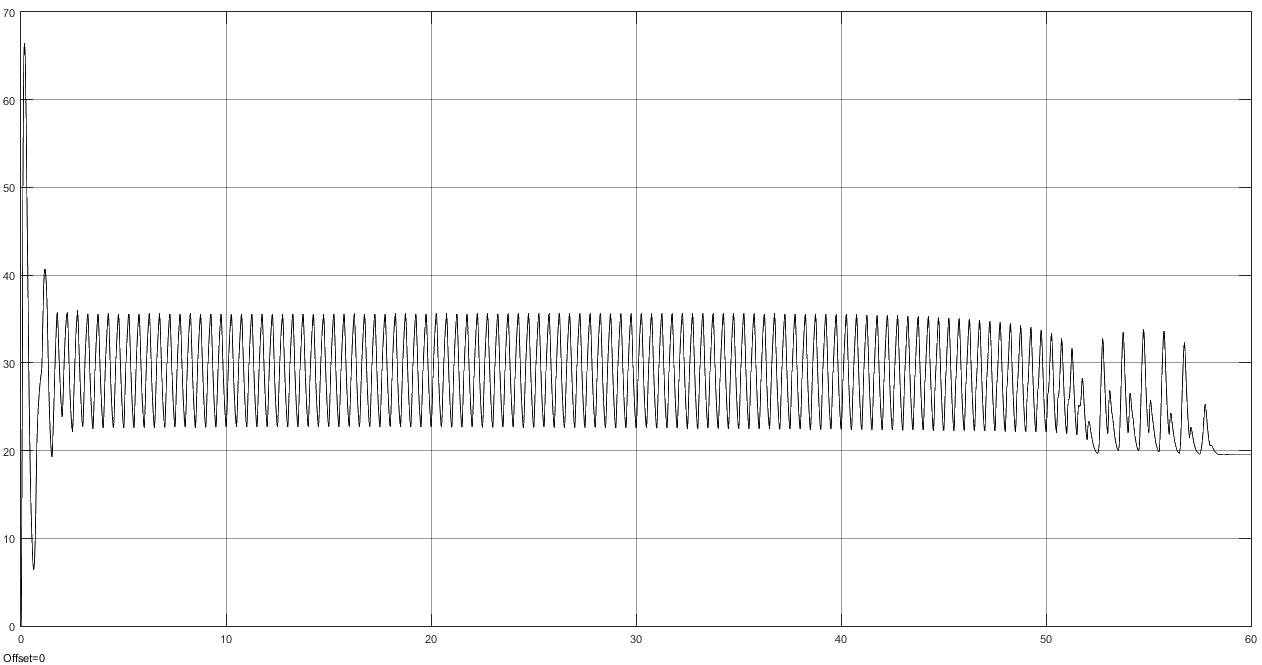
\includegraphics[width = 14 cm, height = 6 cm]{./pics/ResultadoSegundaOrdemEstimativaYcRefB.png}
\caption{Comportamento da saída do modelo da planta de segunda ordem no tempo entre 0 e 60 segundos para a referência b}
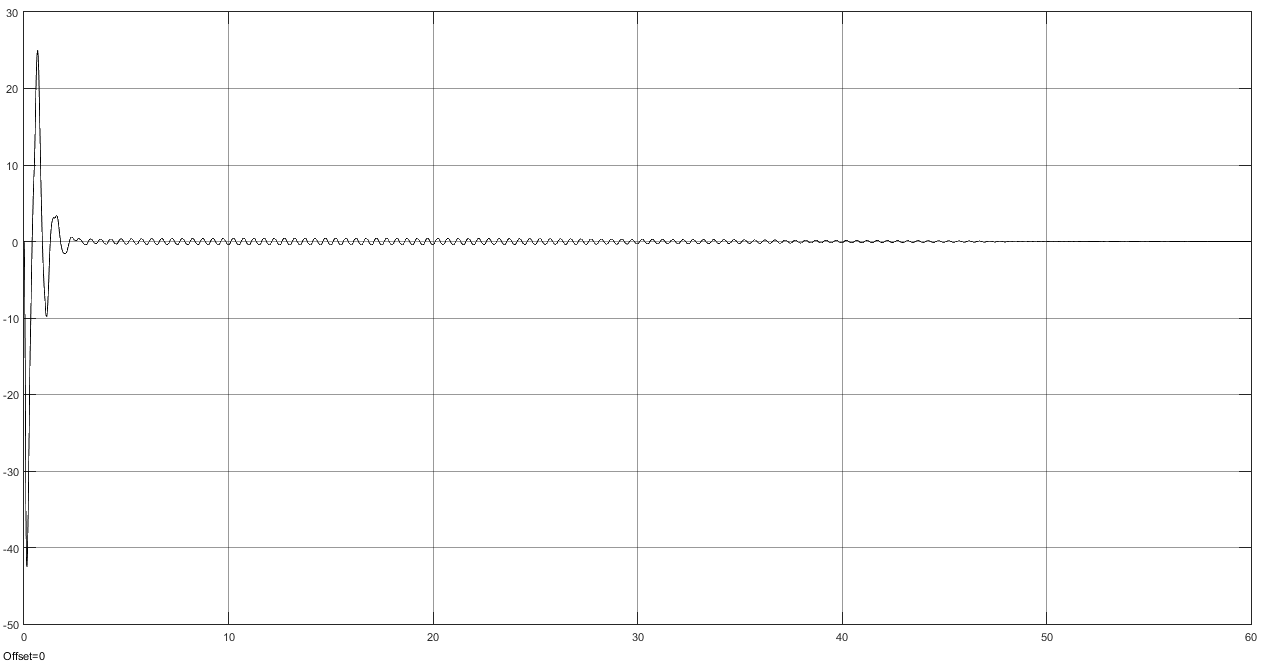
\includegraphics[width = 14 cm, height = 6 cm]{./pics/ResultadoSegundaOrdemEstimativaE0RefB.png}
\caption{Erro de saída da planta de segunda ordem no tempo entre 0 e 60 segundos para a referência b}
\end{figure} 
\begin{figure}
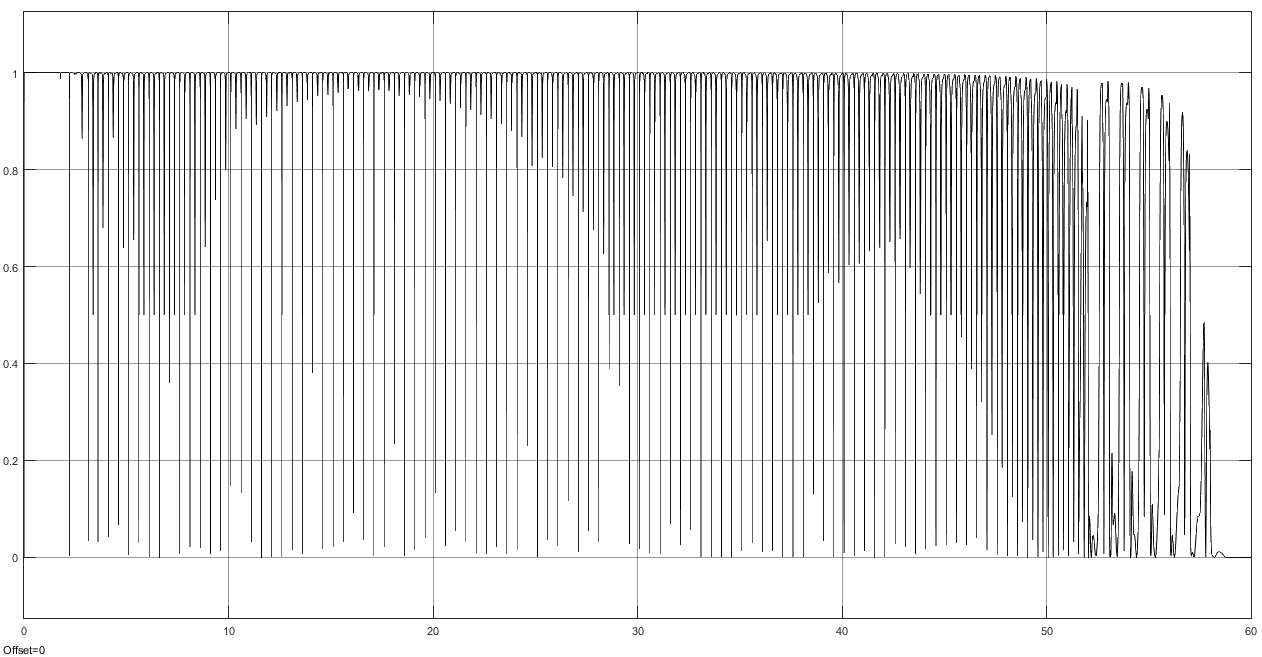
\includegraphics[width = 14 cm, height = 6 cm]{./pics/ResultadoSegundaOrdemEstimativaEpsilonRefB.png}
\caption{Comportamento da figura de mérito $\varepsilon$ para a planta de segunda ordem no tempo entre 0 e 60 segundos para a referência b}
\end{figure}

Aqui, similarmente à planta de primeira ordem, conseguimos convergência dos parâmetros para seus valores verdadeiros, $\hat{\theta_1}=\theta_1^*=39$, $\hat{\theta_2} = \theta_2^* = 200$, $\hat{\theta_3} = \theta_2^* = 30$, (Figuras 30-32) porém sem necessitar que a saída da planta seja oscilante para todo t(Figura 33). Podemos observar a convergência do modelo tanto através do erro de saída(Figura 35), quanto comparando as Figuras 33 e 34. A parte PE do sinal desliga pois a figura de mérito tende a 0 (Figura 36).\\ 

\section{Com Desligamento do Sinal PE, Referência a}


\begin{figure}
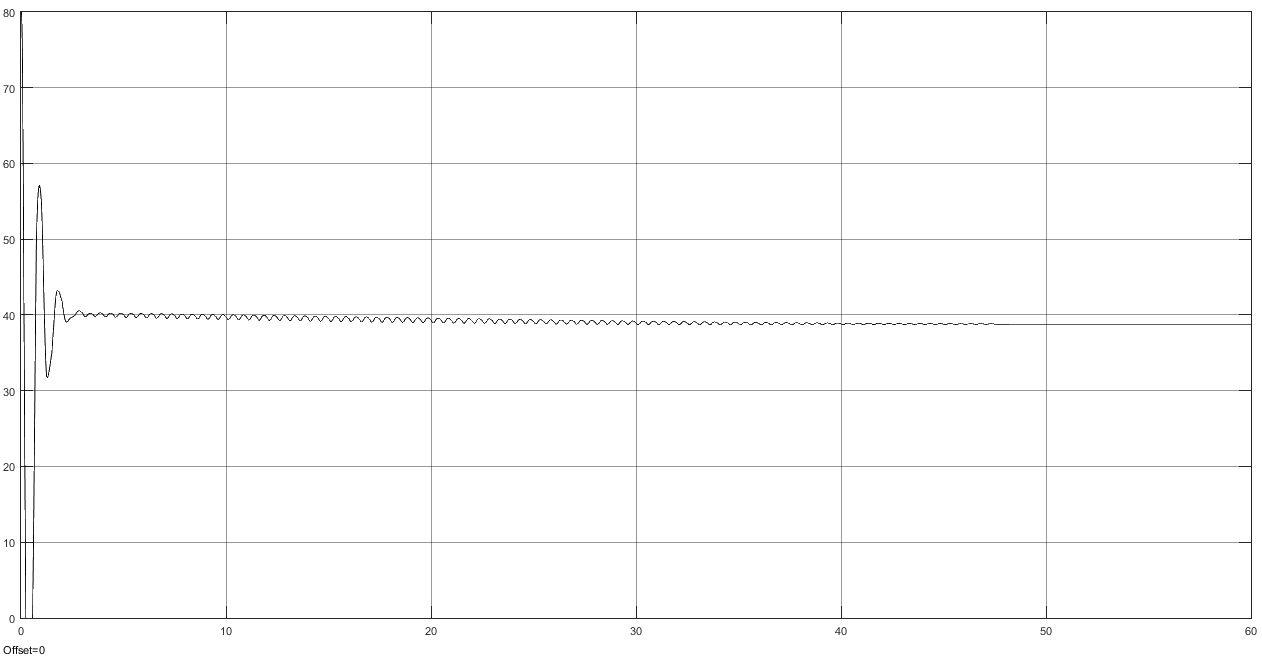
\includegraphics[width = 14 cm, height = 6 cm]{./pics/ResultadoSegundaOrdemEstimativaTheta1RefA.png}
\caption{Comportamento da estimativa $\hat{\theta_1}$ para a planta de segunda ordem no tempo entre 0 e 60 segundos para a referência a}
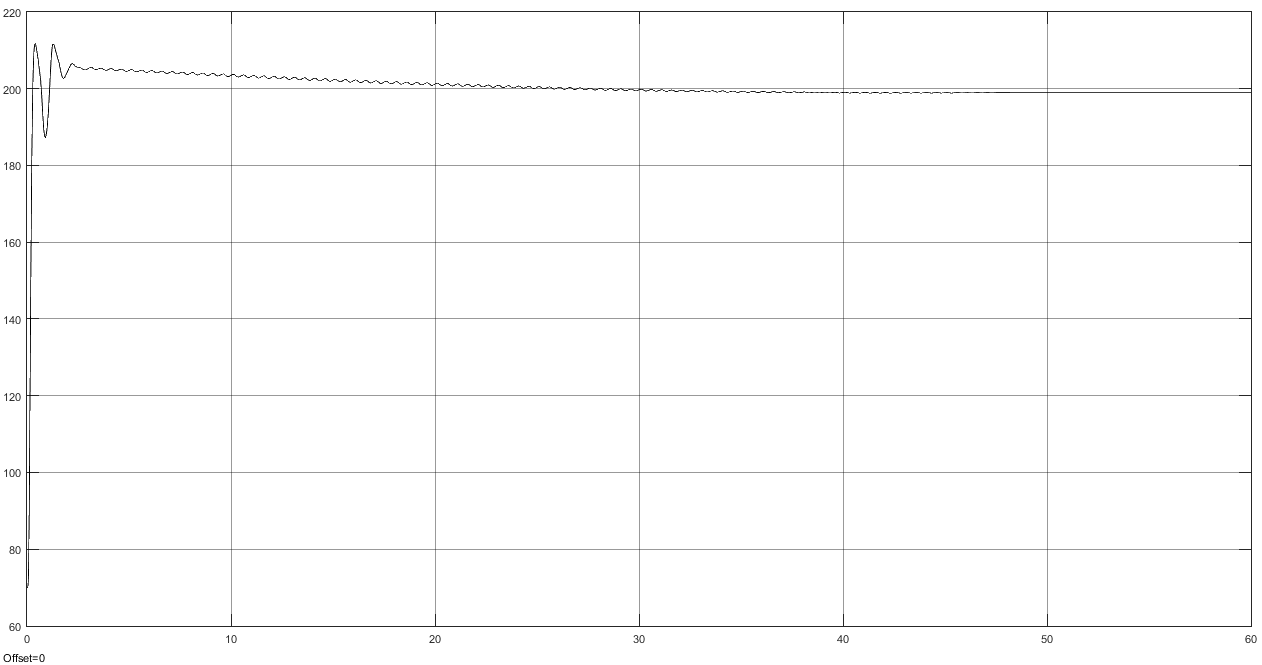
\includegraphics[width = 14 cm, height = 6 cm]{./pics/ResultadoSegundaOrdemEstimativaTheta2RefA.png}
\caption{Comportamento da estimativa $\hat{\theta_2}$ para a planta de segunda ordem no tempo entre 0 e 60 segundos para a referência a}
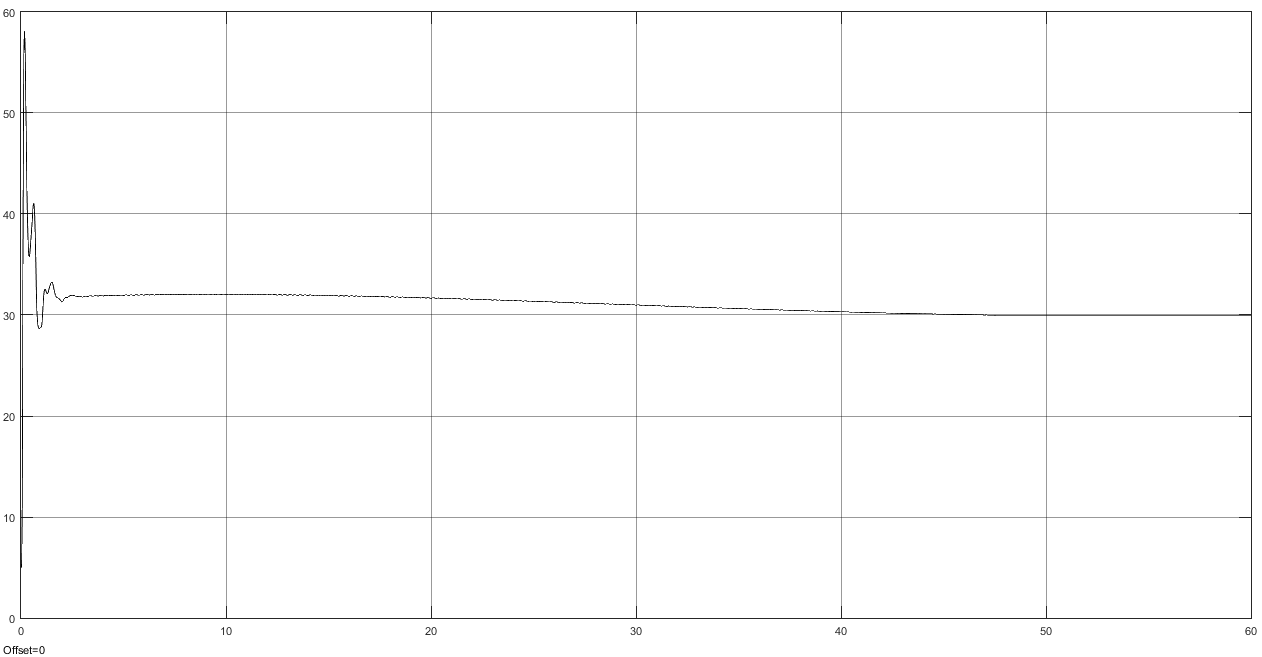
\includegraphics[width = 14 cm, height = 6 cm]{./pics/ResultadoSegundaOrdemEstimativaTheta3RefA.png}
\caption{Comportamento da estimativa $\hat{\theta_3}$ para a planta de segunda ordem no tempo entre 0 e 60 segundos para a referência a}
\end{figure}
\begin{figure}
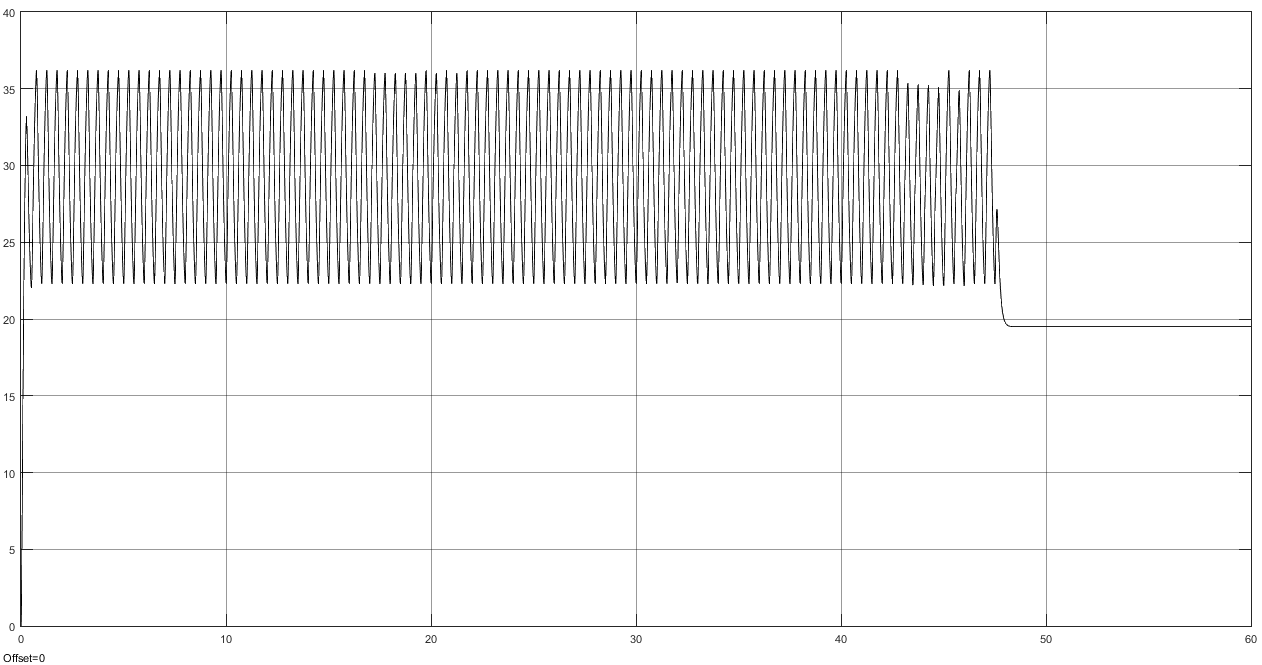
\includegraphics[width = 14 cm, height = 6 cm]{./pics/ResultadoSegundaOrdemEstimativaYRefA.png}
\caption{Comportamento da saída da planta de segunda ordem no tempo entre 0 e 60 segundos para a referência a}
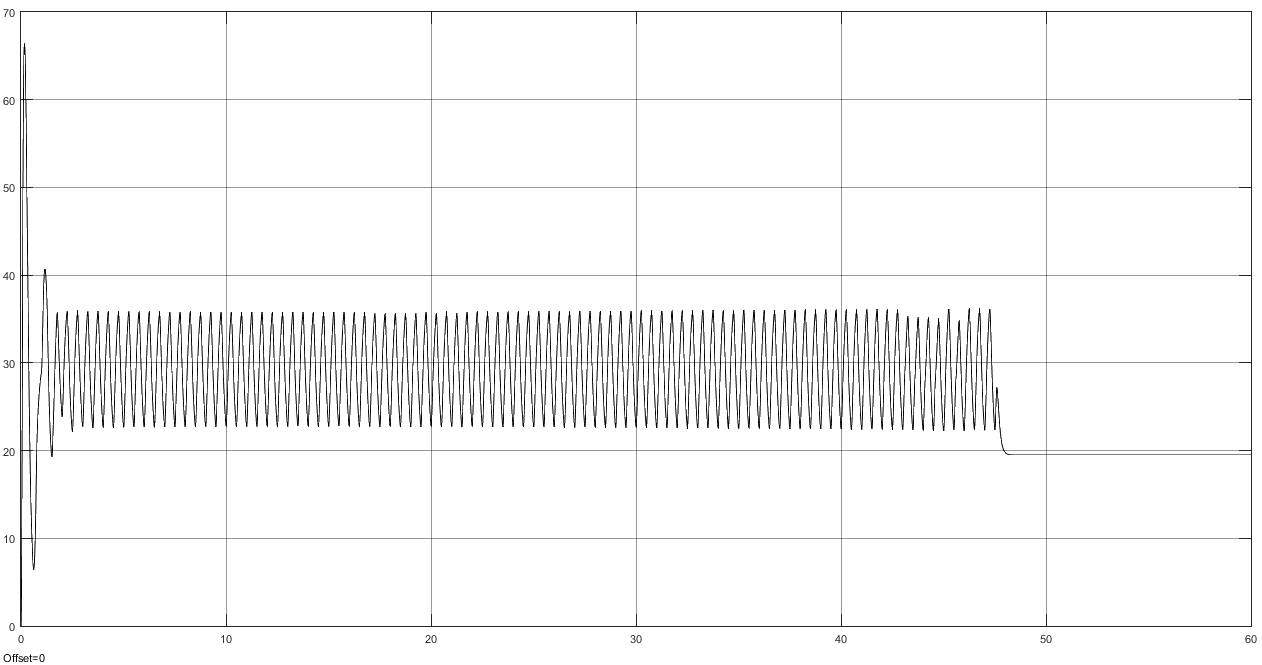
\includegraphics[width = 14 cm, height = 6 cm]{./pics/ResultadoSegundaOrdemEstimativaYcRefA.png}
\caption{Comportamento da saída do modelo da planta de segunda ordem no tempo entre 0 e 60 segundos para a referência a}
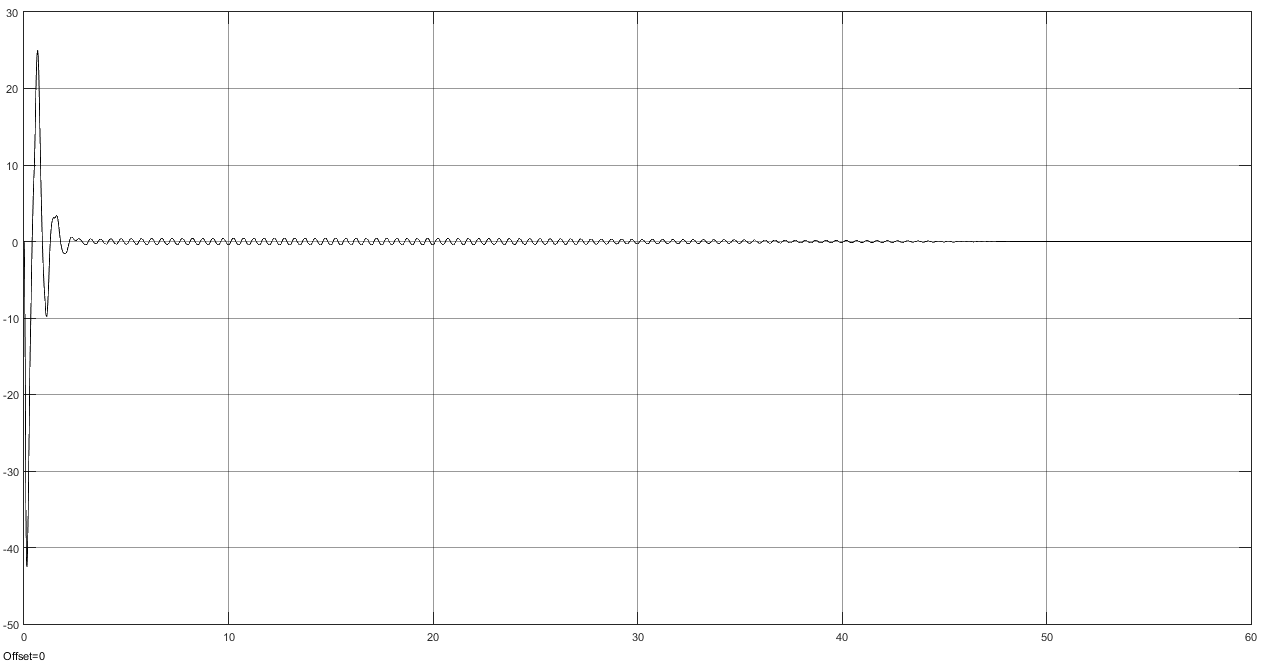
\includegraphics[width = 14 cm, height = 6 cm]{./pics/ResultadoSegundaOrdemEstimativaE0RefA.png}
\caption{Erro de saída da planta de segunda ordem no tempo entre 0 e 60 segundos para a referência a}
\end{figure} 
\begin{figure}
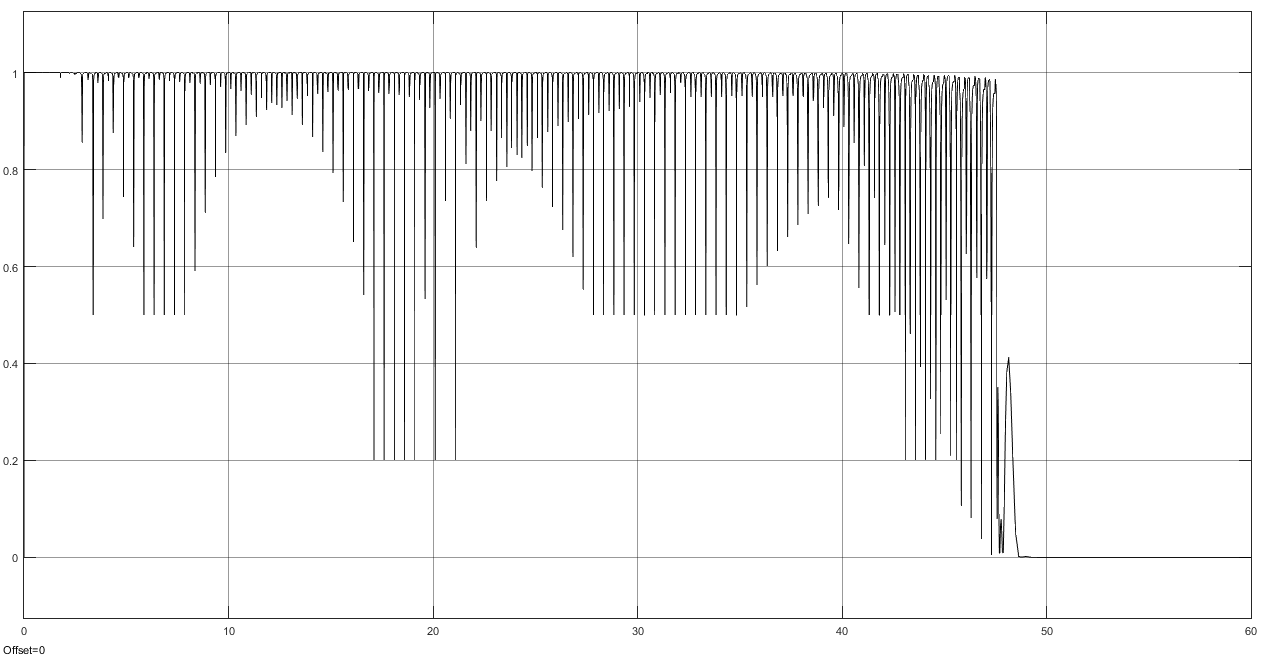
\includegraphics[width = 14 cm, height = 6 cm]{./pics/ResultadoSegundaOrdemEstimativaEpsilonRefA.png}
\caption{Comportamento da figura de mérito $\varepsilon$ para a planta de segunda ordem no tempo entre 0 e 60 segundos para a referência a}
\end{figure}

Com o uso de um relé com amplitude igual a 0.5, conseguimos um resultado similar ao da referência b. Os parâmetros convergem para seus valores verdadeiros, $\hat{\theta_1}=\theta_1^*=39$, $\hat{\theta_2} = \theta_2^* = 200$, $\hat{\theta_3} = \theta_2^* = 30$ (Figuras 37-39). O comportamento do modelo da planta converge (Figuras 40 e 41), pois o erro de saída vai para 0(Figura 42) e a parte PE da referência desliga pois $\varepsilon$ vai para um valor consistentemente menor que a amplitude do relé(Figura 43). Podemos comparar o desempenho para cada referência através da Tabela 3 para o tempo de convergência e da Tabela 4 para a precisão.\\



% Finaliza a parte no bookmark do PDF
% para que se inicie o bookmark na raiz
% e adiciona espaço de parte no Sumário
% ----------------------------------------------------------
\phantompart

% ---
% Conclusão
% ---
\chapter{Considerações Finais}
% ---

Como foi visto no trabalho, a introdução de uma referência c que é persistentemente excitante em relação à planta é capaz de garantir a convergência das estimativas dos parâmetros para seus valores reais, pois a perturbação é suficiente para que se extraia a informação. No entanto, após a convergência dos parâmetros, este tipo de referência se torna contra producente pois produz uma saída da planta que é oscilante, sendo a situação mais comumente desejável no controle de processos que a referência seja um sinal de valor constante e bem definido. De fato, isto se verifica para uma variedade de aplicações, como o controle de velocidade e posição aplicado às áreas de robótica e manufatura industrial.\\

Provamos para as plantas estudadas, através do uso de uma figura de mérito que avalia os valores das taxas de adaptação das estimativas dos parâmetros, que é possível fazer com que a duração do sinal PE seja finita e garanta a convergência das estimativas para seus valores verdadeiros. Para tanto usamos duas referências distintas a e b, onde a referência b usa uma fonte controlada ideal para gerar o sinal a ser introduzido na planta e a referência a usa um relé com amplitude igual a 0.5 para decidir se a parte PE do sinal deve continuar ou não ligada. Este esquema é similar à estratégia implementada em \cite{naval}, onde o erro de saída entre a planta e seu modelo é avaliado para se tomar a mesma decisão. A diferença em relação ao trabalho citado é que embora a avaliação do erro de saída da planta seja uma boa estimativa da convergência do comportamento do modelo para o da planta, as taxas de adaptação possuem mais informação inerente, pois dependem também dos valores dos sinais de entrada da planta e dos ganhos adaptativos escolhidos. Desta forma, mesmo garantindo que o erro de saída está num valor próximo a zero, é possível que a adaptação de um ou mais parâmetros ainda não tenha se completado, especialmente se o valor verdadeiro de cada um destes parâmetros é pequeno em relação aos demais.\\

No futuro seria interessante um estudo mais aprofundado deste esquema de desligamento somada a uma estratégia de controle das plantas estudadas. A figura de mérito introduzida também pode ser estudada como uma forma automática de detectar a convergência dos parâmetros para seus valores reais, adicionando maior confiança às estimativas obtidas. Adicionalmente, a introdução de dinâmicas não modeladas, ruídos e outras perturbações não determinísticas às plantas, além da variação dos valores reais dos parâmetros no tempo também podem ser investigados nestas mesmas plantas ou em plantas de ordem maior que 2 ou com graus relativos diferentes dos usados.\\  

% ----------------------------------------------------------
% ELEMENTOS PÓS-TEXTUAIS
% ----------------------------------------------------------
\postextual
% ----------------------------------------------------------

% ----------------------------------------------------------
% Referências bibliográficas
% ----------------------------------------------------------
\bibliography{abntex2-modelo-references,bib-controleadaptativo}

% ----------------------------------------------------------
% Glossário
% ----------------------------------------------------------
%
% Consulte o manual da classe abntex2 para orientações sobre o glossário.
%
%\glossary

% ----------------------------------------------------------
% Apêndices
% ----------------------------------------------------------

% ---
% Inicia os apêndices
% ---
% ---
\begin{apendicesenv}

\chapter{Tabelas Comparativas}

\begin{table}[htbp]
  \centering
    \caption{Tempo de convergência dos parâmetros, figura de mérito e erro de saída para os valores desejados para a planta de primeira ordem}
    \begin{tabular}{cccc}
    \textbf{Tempo} & \textbf{Referência a} & \textbf{Referência b} & \textbf{Referência c}\\
    $t(\hat{\theta_1}\approx\theta_1^*)$     & $1.67s$ &  $2.70s$ & $2s$ \\
    $t(\hat{\theta_2}\approx\theta_2^*)$     & $1.70s$ &  $2.80s$   & $1.6s$  \\
    $t(\varepsilon\approx 0)$     & $1.65s$ & $2.75s$   & -  \\
    $t(e_0\approx 0$     & $1.63s$& $2.69s$   & $1.9s$  \\  
    \end{tabular}%

    \caption{Precisão de convergência das estimativas dos parâmetros em $t=3s$ para a planta de primeira ordem}
    \begin{tabular}{cccc}
    \textbf{Parâmetro} & \textbf{Referência a} & \textbf{Referência b} & \textbf{Referência c}\\
    $\frac{\hat{\theta_1}}{\theta_1^*}$     & $0.99782$ &  $0.99926$ & $0.99994$ \\
    $\frac{\hat{\theta_2}}{\theta_2^*}$     & $0.99797$ &  $0.99929$   & $0.99990$  \\
    \end{tabular}%

\end{table}

\begin{table}[htbp]
  \centering
    \caption{Tempo de convergência dos parâmetros, figura de mérito e erro de saída para os valores desejados para a planta de segunda ordem}
    \begin{tabular}{cccc}
    \textbf{Tempo} & \textbf{Referência a} & \textbf{Referência b} & \textbf{Referência c}\\
    $t(\hat{\theta_1}\approx\theta_1^*)$     & $39s$ &  $52s$ & $39s$ \\
    $t(\hat{\theta_2}\approx\theta_2^*)$     & $40s$ &  $42s$   & $39s$  \\
    $t(\hat{\theta_3}\approx\theta_3^*)$     & $46s$ &  $54s$   & $55s$  \\
    $t(\epsilon\approx 0)$     & $48s$ & $58s$   & -  \\
    $t(e_0\approx 0$     & $48s$& $57s$   & $50s$  \\  
    \end{tabular}%
 \caption{Precisão de convergência das estimativas dos parâmetros em $t=60s$ para a planta de segunda ordem}
    \begin{tabular}{cccc}
    \textbf{Parâmetro} & \textbf{Referência a} & \textbf{Referência b} & \textbf{Referência c}\\
    $\frac{\hat{\theta_1}}{\theta_1^*}$     & $0.99482$ &  $0.99497$ & $0.99087$ \\
    $\frac{\hat{\theta_2}}{\theta_2^*}$     & $0.99482$ &  $0.99496$   & $0.99719$  \\
    $\frac{\hat{\theta_3}}{\theta_3^*}$     & $0.99940$ &  $0.99607$   & $0.99672$  \\
    \end{tabular}%
\end{table}

\end{apendicesenv}

% ----------------------------------------------------------
% Anexos
% ----------------------------------------------------------

% ---
% Inicia os anexos
% ---
%---------------------------------------------------------------------
% INDICE REMISSIVO
%---------------------------------------------------------------------
\phantompart
\printindex
%---------------------------------------------------------------------


\end{document}
